\documentclass[12pt]{article}
\usepackage{graphicx,booktabs}
\usepackage[utf8]{inputenc}
\usepackage[english]{babel}
\usepackage{float}

\makeatletter
\renewenvironment{abstract}{%
    \if@twocolumn
      \section*{\abstractname}%
    \else %% <- here I've removed \small
      %
        {\bfseries \Large\abstractname\vspace{\z@}}%  %% <- here I've added \Large
      %
      \quotation
    \fi}
    {\if@twocolumn\else\endquotation\fi}
\makeatother


\graphicspath{ {images/} }
\usepackage[letterpaper, portrait, lmargin=1.5in, rmargin=1.25in, tmargin=1in, bmargin=1in]{geometry}
\usepackage{color}
\usepackage{setspace}
\usepackage[titletoc]{appendix}
\usepackage{pdfpages}
\usepackage{booktabs}
\usepackage[nottoc]{tocbibind}
\usepackage{caption}
\captionsetup[figure]{
    position=above,
}
\usepackage{dcolumn}
\usepackage[round]{natbib}
\bibliographystyle{plainnat}
\newcounter{mysubtable}
\usepackage{amsmath}
\usepackage{caption}
\newcommand\modcounter{%
  \refstepcounter{mysubtable}%
  \renewcommand{\thetable}{\thesection.\arabic{table}\alph{mysubtable}}%
}
\newcommand{\appendixnumberline}[1]{Appendix\space}

\let\oldappendix\appendix
\makeatletter
\renewcommand{\appendix}{%
  \addtocontents{toc}{\let\protect\numberline\protect\appendixnumberline}%
  \renewcommand{\@seccntformat}[1]{Appendix~\csname the##1\endcsname\quad}%
  \oldappendix
}
\makeatother

%\makeatletter
%%% The "\@seccntformat" command is an auxiliary command
%%% (see pp. 26f. of 'The LaTeX Companion,' 2nd. ed.)
%\def\@seccntformat#1{\@ifundefined{#1@cntformat}%
%   {\csname the#1\endcsname\quad}  % default
%   {\csname #1@cntformat\endcsname}% enable individual control
%}
%\let\oldappendix\appendix %% save current definition of \appendix
%\renewcommand\appendix{%
%    \oldappendix
%    \newcommand{\section@cntformat}{\appendixname~\thesection\quad}
%}
%\makeatother

    \usepackage{tabularx}
\usepackage{adjustbox}

%\usepackage[toc,page]{appendix}



\doublespacing

\begin{document}

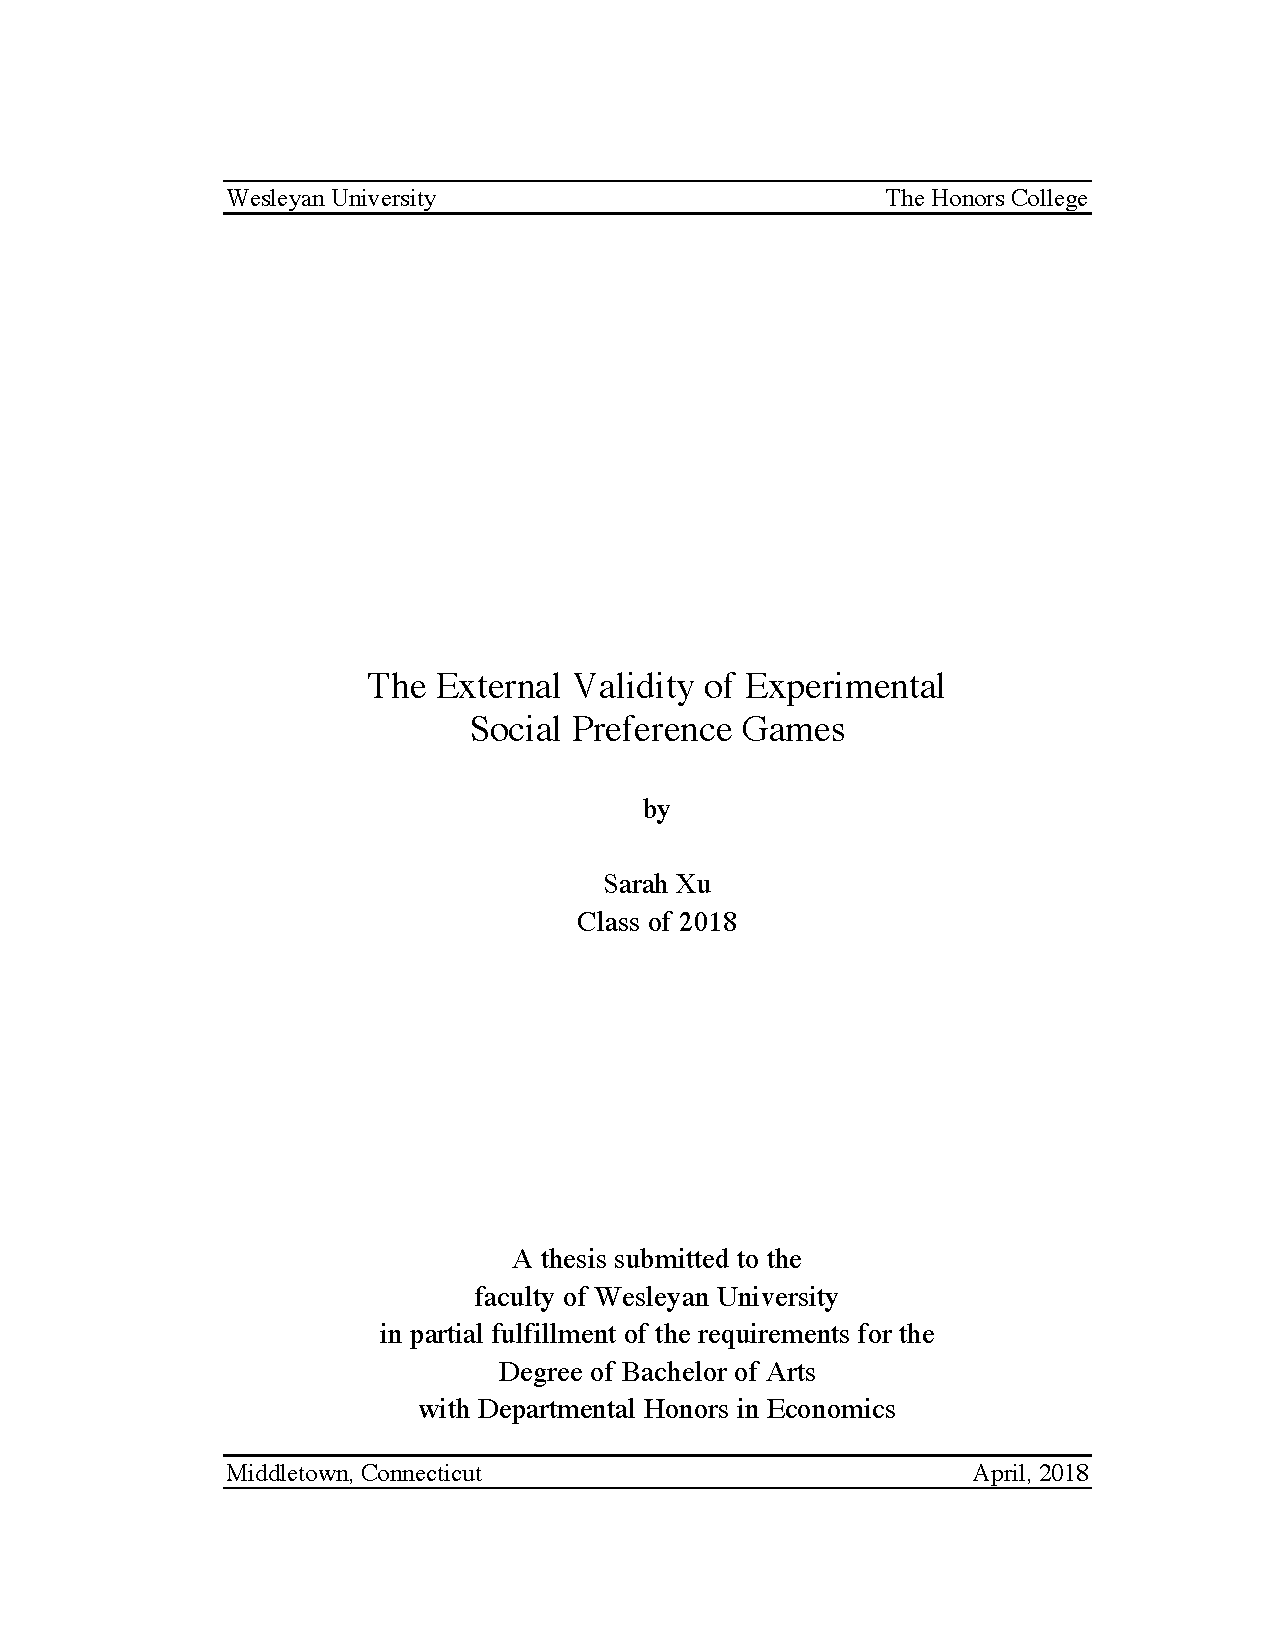
\includepdf[pages=-]{titlepage.pdf}

\newpage
\singlespacing
\tableofcontents
\thispagestyle{empty}


\newpage

\clearpage
\pagenumbering{arabic} 
\section*{Acknowledgements}
\addcontentsline{toc}{section}{Acknowledgements}
Acknowledgements to people


\newpage

\section*{Abstract}
\addcontentsline{toc}{section}{Abstract}

\doublespacing
The external validity of experimental games is a growing topic of interest because researchers commonly use such games to study individuals\rq \ social preferences. Many papers have conducted within-subjects experiments, comparing subjects\rq \ in-lab game decisions to their real-world decisions. However, the current accumulated evidence yields mixed conclusions. Some papers find statistically significant correlations between game and field behavior, while other papers do not. In this research, I compared behavior in various social preference games and self-reported measures regarding past social behavior to a natural, far-removed field measure: donations to Wesleyan University. To examine the explanatory power of social preference games, I ran regression models and looked at the R$^{2}$ values. I also ran various prediction models and compared how well the games predict donations versus randomly guessing. My results show that overall social preference games do a good job in both explaining and predicting donations behavior. However, self-reported measures seem to perform just as well, if not better, than using multiple social preference games. 



\newpage


\doublespacing
\section{Introduction and Literature Review}

The standard economic model assumes individuals\rq \ actions are motivated purely by self-interest. However, from simple observation it is clear that people care about the well-being of others: people volunteer\footnote{The Corporation for National \& Community Service reported 63.6 million volunteers and 7.9 billion hours of service in the U.S. in 2015.}, people donate to causes\footnote{According to Giving USA, individual giving in 2016 was reported to be \$281.86 billion, a 3.9 percent increase from the previous year.}, and social welfare programs exist. If someone is not solely motivated by material self-interest but also cares about the well-being of others, we say that the person has social preferences. 

When studying social preferences, a common approach is to conduct experiments in a laboratory setting. Participants play experimental games, where they receive monetary incentives aligned with the payoffs of the games. Researchers are able to control and influence prices, information, and actions available to the participants, which allows researchers to rigorously target different aspects of social behavior\footnote{Many papers have identified various aspects of social preferences such as altruism, social welfare, inequality aversion, and reciprocity (e.g., \cite{charness_rabin_2002}; \cite{fehr_schmidt_1999}; \cite{rabin_1993}; \cite{fisman_jakiela_kariv_2014}).}.

Study of social preferences with experimental games goes back over twenty years. \cite{forsythe_1994} recruited undergraduate students from the University of Iowa, where the students played dictator and ultimatum games. The dictator game involves a single player (the dictator) who receives an endowment, and the player must choose how to split the amount between themselves and a second player (the receiver). The ultimatum game is a two-player game where the players bargain over a fixed endowment. The first mover (the proposer) divides the sum, and the second mover (the responder) chooses to either accept or reject the offer. If accepted, the proposal is implemented. If rejected, neither player receives any money. Forsythe et al. found that, contrary to the selfish subgame perfect Nash equilibrium in which both dictators/proposers and responders do not send any money, most players did share proportions of their endowments.

\cite{berg_1995} recruited undergraduate students from the University of Minnesota to participate in trust games. The trust game is a two-player game. Similar to the ultimatum game, the proposer receives an endowment and proposes how to divide the endowment between themselves and the second mover. The offered amount is multiplied by a factor, and the responder decides how much of the multiplied contribution to return to the proposer. The authors found that participants showed high levels of trust and reciprocity: 94\% of the proposers sent money, and over one-third of the responders returned an amount greater than what was given to them.

 \cite{hermann_thoni_gachter_2008} conducted public goods experiments across 16 participant pools. The public goods game is an N-player game where each player receives the same sum of money and simultaneously decides how much to put into a public fund. The total amount in the public fund is multiplied by a factor, and divided evenly amongst the players. Hermann et al. found that that varying opportunities for punishment led to varying cooperation levels.

Using social preference games has become one of the building blocks of experimental and behavioral economics. However, pro-social behavior may be influenced by a variety of non-monetary factors, leading to variation in game behavior. One issue is that the subjects\rq \ actions are under the scrutiny of the researcher. For example, \cite{hoffman_1994} found that almost 50\% of their subjects donated at least \$3 (out of a \$10 pie) when playing the dictator game. However, when the authors implemented a ``double-blind'' treatment where both the experimenter and other subjects could not observe the dictator\rq s actions, they found that only 16\% of subjects gave at least \$3.

Individuals are also influenced heavily on the framing of the situation. In a trust game, \cite{burnham_mccabe_smith_2000} switched between calling the responder as ``partner'' or ``opponent'', and found that trustworthiness with ``partner'' was over twice that for ``opponent''. Similarly, \cite{ross_ward_1996} found that participants showed high levels of cooperation when playing a prisoner\rq s dilemma game called a ``community'' game, and participants showed lower levels of cooperation when the game was called a ``Wall Street'' game. 

Some studies also found that varying the level of stakes led to significantly different behaviors. \cite{carpenter_verhoogen_burks_2005} discovered that increasing the stakes from \$10 to \$100 decreased the median offer in the dictator game from 40\% of the endowment to 20\%, and \cite{slonim_roth_1998} found that in the ultimatum game, rejections occurred less frequently and proposal amounts decreased as stakes increased. However, \cite{cherry_frykblom_shogren_2002} found no significant differences in offer amounts when increasing the stakes from \$10 to \$40 in the dictator game. 

On a larger scale, experiments conducted in a lab setting are abstract and remote from realistic situations, so there may also be non-monetary factors that lead to varying behaviors between lab setting and real-world setting. For example, people know their actions are being recorded during an experiment. However, when making real-life choices, their decisions are made in private. Thus people may be more pro-social in the lab than they are in real life. On the other hand, real-life situations may have more personal meaning to the individual than experimental games do. In this case, people could be more pro-social than they portray in the lab. As such, actions made in a lab setting may not reflect the individual\rq s real-world behavior\footnote{See \cite{levitt_list_2007} for a full discussion of factors, with supporting literature, that may lead to deviations between game behavior and real-world behavior.}. Therefore an important question is the external validity of social preference games -- that is, the extent to which decisions made in the games can be generalized to decisions made in the field.

Some studies found that game behavior does explain field behavior. \cite{baran_2010} compared MBA alumni donations to their university with their reciprocity behavior when playing the trust game. The authors found that responder behavior predicted university donations. \cite{franzen_pointner_2012} compared decisions from university students participating in standard dictator games to their actions when receiving a misdirected letter containing money, and found that subjects who showed pro-social behavior in the lab returned the misdirected letters more often than subjects who were selfish in the lab. \cite{englmaier_gebhardt_2011} conducted field experiments where they compared university students\rq \ free riding behavior at the library to free riding behavior in a public goods game, and found statistically significant correlation between field and lab measures. There are also studies that used non-student subjects: \cite{fehr_leibbrandt_2011} conducted public goods games with Brazilian fishermen, and found that those who were more cooperative in the games were also less likely to exploit the communal fishing grounds. \cite{karlan_2005} compared subjects\rq \ trust game behavior to their loans repayment behavior in a Peruvian microfinance program, and found that those who showed ``trustworthy'' behavior were less likely to default on their loans. 

On the other hand, a number of papers found lab behavior had no explanatory power for field behavior. \cite{goeschl_2015} examined university students\rq \ behavior in two different tasks: a public goods game and their contributions to a field situation about reducing CO$_{2}$ emissions. The authors found that decisions in both tasks were uncorrelated. \cite{hill_gurven_2004} carried out ultimatum and public goods games on Paraguay Ache Indians. They compared the game behaviors to observed food production and sharing patterns with individuals outside the nuclear family, and found no significant relationship to lab behavior. \cite{gurven_winking_2008} recruited Tsimane forager-horticulturalists in Bolivia, and compared behavior when playing dictator and ultimatum games to their food-sharing behavior. The authors concluded no relation between the two measures. \cite{voors_2012} used farmers in Sierra Leone, and compared their decisions in a public goods game to their decisions when asked to contribute to a real community public good. They found no meaningful correlation in behavior between the lab and field measures. 

\cite{galizzi_navarro-martinez_2017} summarized that about 40\% of reported correlations between lab and field behavior and regressions found statistically significant associations\footnote{See Galizzi and Navarro-Martinez for their full systematic review and meta-analysis of literature on within-subjects lab-field studies.}. Therefore it is clear that the current evidence for the external validity of experimental games is mixed. Galizzi and Navarro-Martinez noted, however, that the previous studies compared only one social preference game to one specific field measure. The theoretical nature of the games makes it difficult to conceptually map them to a specific field measure, and so it is crucial to have a more systematic approach. The authors conducted their own study where participants answered questions about social behaviors exhibited in the past, played various social preference games, and encountered naturalistic field situations. The field situations included a research assistant asking for help carrying boxes down the stairs, asking to use the participant\rq s phone to make a brief phone call, asking for donations to a children\rq s charity, asking for donations to an environmental charity, or asking for donations to the lab\rq s research fund.  The authors\rq \ overarching conclusion was that behavior when playing the experimental games does a poor job predicting both the survey questions and the field behaviors, but that more systematic studies are needed in order to draw a definite conclusion. This is where my thesis contributes.

My research contributes to the ongoing discussion on the external validity of social preference games by providing another systematic study. I recruited Wesleyan University seniors and recent alumni to play various experimental games. I also had the participants answer self-reported questions regarding their past social behavior as an additional layer to evaluate the predictive ability of the games, and I used donations to Wesleyan University as the field measure.

{\color{red}My results show that social preference games explain little to none of the donations behavior. In fact, the self-reported measures seem to perform just as well as the games. In addition, self-reported measures seem to play a more important role when predicting the field measure.}



\section{Methods}

Each participant was presented with two sets of tasks: (i) incentivized social preference games, and (ii) self-reported questions regarding past social behavior. The field measure used to compare to participants\rq \ lab results was their donations to Wesleyan University.  In addition, I examined which tool -- the social preference games, the self-reported measures, or both -- performed better at predicting the donations behavior.
 
Wesleyan University seniors and recent alumni received an invitation email briefly explaining my research and asking for participation in my study (2,004 emails were provided by Wesleyan University Relations). The entire study was computerized, programmed and implemented using Qualtrics. Online links to both the experimental games and survey questions were provided so that those who chose to take part completed the study remotely (which minimized scrutiny and thereby reduced the risk for exaggerated behavior). Participants received an overview of the two tasks they would complete, and were informed that upon completion of the study, their major, class year, and Wesleyan donations information would be collected.

In order to incentivize completion of both the games and survey questions as well as elicit honest game behavior, participants were informed that completing the entire study made them eligible for a lottery prize. All of the games used ``tickets" as the experimental currency unit, where the total tickets each participant earned in the games equaled how many lottery tickets they owned. After the participation deadline passed, ten tickets were randomly drawn and each winner received \$100.


\subsection{Incentivized social preference games}

%Those who chose to participate in the study received a unique identifier assigned by Qualtrics.

Participants first played four social preference games (in random order): the generalized dictator game, the ultimatum game, the trust game, and the public goods game. Before each game, they received detailed instructions along with an example to illustrate how each game worked. For the ultimatum and trust games, each participant had the opportunity to play the roles of both proposer and responder. At the end of the participation deadline, all participants were randomly paired and ticket payoffs were calculated.

Below are descriptions of each game the participants played, along with examples (see Appendix C for screenshots of each game, along with respective instructions and examples, from the online online study). In addition, I describe the decisions individuals are expected to make depending on various preferences they may have.

\subsubsection{Generalized dictator game}

Each participant, playing as the dictator, played nine different rounds of the generalized dictator game\footnote{The design is based off of the study by \cite{andreoni_miller_2002}.}. In each round, participants were given different endowments and prices of giving, and were asked how they would like to divide the endowment with an anonymous, random Player 2. Therefore the budget constraint is given by \(\pi_{s} + p\pi_{o} = \textit{m}\), where \(\pi_{s}\) is how many tickets were kept, \(\pi_{o}\) is how many tickets were given, \(p\) is the relative price of giving, and \textit{m} is the endowment. The endowment in each round was either 10, 12, or 15 tickets. Every ticket the participant kept was worth either 1, 2, 3, or 4 tickets (hold price), and every ticket given to Player 2 was also worth either 1, 2, 3, or 4 tickets (pass price). Below are the nine sets of endowments and prices of giving used in the study:


\begin{center}
\begin{tabular}{ c c c c c }
\hline \hline
 Budget & Ticket Endowment & Hold Price & Pass Price & Relative Price of Giving \\ 
 \hline
1 & 15 & 1 & 2 & \(\frac{1}{2}\)  \\  
2 & 10 & 1 & 3 & \(\frac{1}{3}\)  \\  
3 & 15 & 2 & 1 & 2 \\  
4 & 12 & 1 & 2 & \(\frac{1}{2}\)  \\  
5 & 10 & 3 & 1 & 3  \\  
6 & 15 & 1 & 1 & 1  \\  
7 & 12 & 2 & 1 & 2 \\  
8 & 10 & 4 & 1 & 4 \\  
9 & 10 & 1 & 4 & \(\frac{1}{4}\)  \\ 
\hline \hline \\
\end{tabular}
\end{center}


Participants were given the endowment and hold/pass price for each round, and were presented an interactive slider bar that displayed the different ticket amounts each player could earn. The slider bar ensured choices fulfilled the budget constraint, and eliminated the need to perform calculations by directly showing how many tickets each player would receive.

\textit{Example:} Divide 10 tickets: Hold @ 1 ticket each, Pass @ 3 tickets each. In this example, the endowment is 10 tickets, and the relative price of giving is \(\frac{1}{3}\). That is, however many tickets the player decides to keep is multiplied by 1 (the hold price), and however many tickets given to Player 2 is multiplied by 3 (the pass price). The player is presented a slider bar, ranging from giving 0 tickets to giving 10 tickets, and with each possible offer amount, the player was told the total ticket amounts received by both players in the form (total tickets received, total tickets given). For example, if the player decides to give 4 tickets to Player 2, they would see (6, 12) which means they would receive 6 tickets (10 - 4 = 6) and Player 2 would receive 12 tickets (4 * 3 = 12).

\underline{Selfish preferences:} If the individual has selfish preferences, their utility function is given by U(\(\pi_{s}\), \(\pi_{o}\)) = \(\pi_{s}\). The individual will prefer to maximize their own payoff, so their optimal allocation is to keep their entire endowment.

\underline{Rawlsian preferences:} Individuals with Rawlsian preferences have their utility represented by U(\(\pi_{s}\), \(\pi_{o}\)) = \(\min(\pi_{s}, \pi_{o})\). The optimal allocation is to evenly split the endowment, i.e. \(\pi_{s}\) = \(\pi_{o}\) = 5 tickets.

\underline{Utilitarian preferences:} If the individual has utilitarian preferences, their utility is U(\(\pi_{s}\), \(\pi_{o}\)) = \(\pi_{s}\) + \(\pi_{o}\). The individual will prefer to allocate all payoffs to whichever \(\pi_{s}\) or \(\pi_{o}\) is cheaper. That is, if \(p\) $<$ 1 they will send their entire endowment to the other player, and if \(p\) $>$ 1 they will keep their endowment.



\subsubsection{Ultimatum game}

\textbf{Player 1:} Each participant was endowed with 10 tickets, and were told to decide how much of their endowment to send to an anonymous, random responder (Player 2) so that \(\pi_{s} + \pi_{o} = 10\). They were also informed that the responder may or may not reject the proposed allocation: if the allocation is accepted, then the proposal is implemented (Player 1 will receive \(\pi_{s}\) and Player 2 will receive \(\pi_{o}\)), and if the allocation is rejected, neither player receives any tickets.

\textit{Example:} Suppose the participant chooses to give 3 tickets to Player 2. If Player 2 accepts the proposal, the participant will receive 7 tickets (10 - 3 = 7) and Player 2 will receive 3 tickets. However, if Player 2 does not like the proposal and rejects the proposition, then both players will receive 0 tickets.
 
\textbf{Player 2:} Each participant was informed that the proposer (Player 1) was given an endowment of 10 tickets. They were presented a list from 0 tickets to 10 tickets (in 1-ticket increments), which represented the different amounts that Player 1 could choose to send. The participants were instructed to indicate whether they accept or reject each hypothetical proposal, and were told that accepting means they agree to receiving the offered amount, and rejecting means they do not agree and instead both players will receive 0 tickets.

\textit{Example:} Suppose the participant chooses to reject all offered amounts below 5 tickets, and accept all offered amounts equal to or greater than 5 tickets. If Player 1 chose to offer 3 tickets, then both players will receive 0 tickets. Or if Player 1 chose to offer 6 tickets, then Player 1 will receive 4 tickets (10 - 6 = 4) and the participant will receive 6 tickets.

\underline{Selfish preferences:} Selfish responders should never reject a non-zero offer. If selfish proposers assume responders are also selfish, they will offer the smallest non-zero amount (in this case, 1 ticket). However, if the proposers believe the responders are not purely selfish and will reject small amounts, then they will offer the smallest non-zero amount they believe will be accepted. For example, if the proposer believes the responder has Rawlsian preferences (i.e. the responder will reject offers below half the endowment) then the proposer will offer 5 tickets.

\underline{Fehr-Schmidt difference-aversion preferences:} Responders may care about both inequality and total welfare:\\

$ U(\pi_{s}, \pi_{o})  = \begin{cases}
      \pi_{s} - \alpha(\pi_{s} - \pi_{o}) & \text{if }\pi_{s} > \pi_{o} \\
      \pi_{s} - \beta(\pi_{o} - \pi_{s}) & \text{if }\pi_{s} \leq \pi_{o}
    \end{cases}\, $ \\

\noindent where $ 0 \leq \alpha \leq \beta \leq 1$. That is, the responder dislikes inequality but dislikes it even more if they have the smaller allocation. For example, say $\alpha = \frac{1}{2}$ and $\beta=1$. Compared to the utility of rejecting (U(\$0, \$0)=0), the responder will accept payoffs (\$4, \$6) since U(\$4, \$6) = 4 - 1(6 - 4) = 4 - 2 = 2, but reject payoffs (\$3, \$7) since U(\$3, \$7) = 3 - 1(7 - 3) = 3 - 4 = -1.

	
\subsubsection{Trust game}
\textbf{Player 1:} Each participant was endowed with 10 tickets. They were prompted to decide how much of their endowment to send to an anonymous, random responder (Player 2) so that \(\pi_{s} + \pi_{o} = 10\). The participants were told that the amount sent over would be multiplied by 3, i.e. Player 2 would receive 3\(\pi_{o}\), and that Player 2 would then decide how many tickets, r \(\leq 3\pi_{o}\), they would like to return. Overall, Player 1 received \(\pi_{s}\)+r tickets and Player 2 received 3\(\pi_{o}\) - r tickets.

\textit{Example:} If the participant chooses to send 5 tickets, then Player 2 will receive 15 tickets (5 * 3 = 15). Player 2 will then decide how many tickets to return. If Player 2 chooses to send back 3 tickets, then Player 1 will earn a total of 8 tickets (5 + 3 = 8) and Player 2 will earn 12 tickets (15 - 3 = 12).

\textbf{Player 2:} Each participant was informed that the proposer (Player 1) received an endowment of 10 tickets. They were then given a list of all ten possible multiplied amounts that Player 1 could have chosen to send, ranging from 3 tickets to 30 tickets in 3-ticket increments. For each possible offered amount, the participants were prompted to enter the number of tickets they would like to return back to the proposer. They were given clear instructions that their input could not exceed what was given to them. For example, if Player 1 gave them a multiplied amount of 15 tickets, then the maximum number of tickets the participant could return is 15 tickets.

\underline{\textit{Example:}} Suppose the participant\rq s return scheme is as below: \\
	
\begin{center}
\begin{tabular}{ c c }
\hline \hline
 Possible Offer Amounts (Multiplied) & Tickets Returned \\ 
 \hline
3 & 0  \\  
6 & 1 \\  
9 & 3  \\  
12 & 3  \\  
15 & 5   \\  
18 & 5  \\  
21 & 5 \\  
24 & 5 \\  
27 & 5 \\  
30 & 5 \\  
\hline \hline \\
\end{tabular}
\end{center} 


where the first column is a list of all possible multiplied amounts that Player 1 could choose to send, and the second column indicates how many tickets the participant would like to return. If Player 1 decided to give 7 tickets to the participant, then the participant will receive a multiplied amount of 21 tickets (7 * 3 = 21). As indicated by the participant\rq s return scheme, the participant chose to return 5 tickets. Thus Player 1 receives 8 tickets (3 + 5 =  8), and the participant receives 16 tickets (21 - 5 = 16).

\underline{Selfish preferences:} Purely selfish responders should return nothing. If purely selfish proposers assume responders are also purely selfish, then they will pass nothing. However, the proposers may pass a portion of their endowment if they believe the responders will return an amount greater than what was sent to them.


\underline{Utilitarian preferences:} Proposers with utilitarian preferences will to maximize the sum of payoffs. Since the amount sent to the responder is multiplied by a positive factor, they will send their entire endowment to the responder. This can also be seen mathematically:

U(\(\pi_{s}\), \(\pi_{o}\)) = \(\pi_{s}\) + \(\pi_{o}\)

\hspace{17mm} \( = \pi_{s} + r + 3\pi_{o} - r \)

\hspace{17mm} \( = \pi_{s} + 3\pi_{o} \)

The amount sent increases the proposer\rq s utility more than the amount kept, so the proposer will choose to send everything to the responder.
	
\subsubsection{Public goods game}

Each participant was given 10 tickets, and told that they would be randomly matched with one other player. They were then prompted to decide how much of their endowment to contribute to a group fund, and were informed that the other player was told to do the same task. The total tickets in the group fund was multiplied by 2, and divided evenly between the two players. Therefore each player received the remaining amount of their endowment plus the divided amount from the public fund. The payoff function is given by \( P_{i} = 10 - g_{i} + \sum_{n=1}^{2} g_{n}\) where \(g_{i}\) is the amount that player \textit{i} donated to the fund, and \(\sum_{n=1}^{2}g_{n}\) is the sum of both players\rq \ donations to the public fund.

\textit{Example:} Suppose the participant chooses to contribute 3 tickets, and the second player chooses to contribute 5 tickets. The total donated amount, \(\sum_{n=1}^{N} g_{n}\), is 8 tickets. Therefore the participant receives \( P_{1} = 10 - 3 + 8  = \) 15 tickets, and the second player receives \( P_{2} = 10 - 5 + 8 = \) 13 tickets 

\underline{Selfish preferences:} Player 1\rq s payoff function is:

\( P_{1} = 10 - g_{1} + \sum_{n=1}^{2} g_{n} \)

\hspace{4mm} = \(10 - g_{1} + g_{1} + g_{2} \)

\hspace{4mm} = \(10 + g_{2}\)

\noindent and Player 2\rq s payoff function is:

\( P_{2} = 10 - g_{2} + \sum_{n=1}^{2} g_{n} \)

\hspace{4mm} = \(10 - g_{2} + g_{1} + g_{2} \)

\hspace{4mm} = \(10 + g_{1}\)

Each player\rq s payoff depends on the other player\rq s contribution, and so selfish players will not send any tickets into the public fund.

\underline{Utilitarian preferences:} From the perspective of Player 1, their utility equals the sum of both players\rq \ payoffs:

\(U_{1} = P_{1} + P_{2}\)

\hspace{4mm} = \(10 + g_{2} + 10 + g_{1}\)

\hspace{4mm} = \(20 + g_{1} + g_{2}\)

Players with utilitarian preferences will send their entire endowment into the public fund.


\subsubsection{Strategy Method}

Since the participants were completing the games at their own availability, they were randomly matched with other participants after all data had been collected. In the two-player games (ultimatum and trust games) which required both a proposer and responder, each participant played as both roles. When playing as the proposer, the participant decided how to split the endowment. When playing as the responder, the participant saw a list of all possible offer amounts and was prompted for their choice for each offer. This is called the strategy method.

There are several reasons why the strategy method is advantageous. First, it is useful to have all of the responder\rq s potential choices so that payoffs can be determined after the fact. Most importantly, the strategy method gives more information. If players were matched with other players live, then we would only have the responder\rq s response given the proposer\rq s offer. The strategy method, however, provides all returned amounts for all possible donated amounts in the trust game, and provides participants\rq \ minimum accepted amount in the ultimatum game. 

\subsubsection{Payment}

Participants were randomly paired, and ticket payoffs were determined for each game. In each assigned pair, one participant was randomly selected to be Player 1 (i.e. they were the dictator in the generalized dictator game, and proposer in both the ultimatum game and trust game), and the other was Player 2 (i.e. they were the receiver in the generalized dictator game, and the responder in both the ultimatum and trust game). I ran through each game and calculated ticket payoffs for each participant. Since the generalized dictator game consisted of nine rounds, one round was randomly selected; each participant received the tickets based on their decision for that round. 

After each participants\rq \ total lottery tickets were calculated, ten tickets were drawn. Each ticket owner was emailed instructions on how to receive their \$100 prize through direct deposit or check. 

\subsection{Self-reported measures of past social behaviors}

Participants then reported on past pro-social behavior. The questions were adapted from the Self-Report Altruism (SRA) scale introduced by \cite{rushton_chrisjohn_fekken_1981}. The survey was comprised of 10 items, and participants reported how frequently they have done each item. Participants rated each statement as either ``Never'', ``Once'', ``More than once'', ``Often'', or ``Very often''. Examples included ``I have donated money at the cash register when buying groceries'' and ``I have pointed out a clerk\rq s error (at the supermarket, at a restaurant) in undercharging me.'' A full list of the items from the online study is displayed in Appendix D. 

\subsection{Field Measure}

After the participation deadline passed, Wesleyan University Relations provided a dataset that contained each participant\rq s Wesleyan donations information.

There are several reasons why I chose to use donations as my field measure. First, many behavioral economics papers that explored the relationship between in-lab behavior and field behavior used donations\footnote{See, e.g., \cite{benz_meier_2006}; Baran et al.; Falk et al.}. \cite{falk_2013} justified that donations are an accurate field measure because they do not rely on self-reported responses but on actual decisions. Furthermore, donations are made in private and never made public, and students/alumni are unaware that their actions will be analyzed in a future research study. The lack of scrutiny therefore indicates donations should reflect the donors\rq \ genuine altruism. The authors then pointed out the most important reason for their decision to use donations: all students and alumni are solicited, so everybody has to make the decision about donating.

In addition, donations are a more accurate field measure than creating a scenario at the end of the online session. I previously mentioned that in the experiment by Galizzi and Navarro-Martinez, participants were subject to the experimenter demand effect: because participants encountered the field experiments shortly after completing the lab experiments, it would not be difficult for participants to link the two situations together. Therefore, participants could have acted more pro-socially than they would usually under normal circumstances. At Wesleyan University, seniors are solicited for donations around once per semester. Alumni are typically solicited for donations at the end of November / beginning of December, March, and June. The online study in this research was released between solicitation cycles for both seniors and recent alumni (early January 2018), and participants\rq \ donations information were provided as of January 2018. Therefore participants\rq \ donations are not influenced by the experimenter demand effect.


\subsubsection{Theoretical Correspondences Between Games and Donations}

All of the social preference games I chose for my study tap into different types of pro-social behaviors that are also related to donating. First, the dictators in the generalized dictator game, proposers in the ultimatum and trust games, responders in the trust game, and players in the public goods game have the option to keep their endowment to themselves, but may also choose to share their endowment with another person. Therefore the actions in these games can be explained by altruism: those who choose to keep their endowment exhibit lower levels of altruism, and those who choose to share their endowment demonstrate higher levels of altruism. Likewise, altruism is the most common representation for donating since the donor chooses to give their income to the university to benefit future students. 

Proposers\rq \ decisions in the trust and public goods games indicate their trust levels. In the trust game, since the proposers\rq \ offerings get multiplied by a factor, the proposers may exhibit trust by sharing their endowment with the hopes of the responders sending back an amount larger than what was given. Similarly, in the public goods game, players can possibly receive a net amount larger than their initial endowment if the other players contribute into the public fund. Thus, players may show trust by sending some of their endowment with the hopes that the other players will do the same. Correspondingly, donating may also represent trust since donors are trusting that the University will use their donations to benefit future students.

Responders\rq \ actions in the trust game can also be interpreted by reciprocity: if the proposers decided to share their endowment, the responders then has the opportunity to give back to the proposers. The responders display higher levels of reciprocity if they return some of what was first given to them, and display lower levels of reciprocity if they give back little or nothing. The responders\rq \ actions can also be represented by trustworthiness: the proposers may contribute some of their endowment in hopes of the responders returning a larger amount than what was offered. Thus responders who return a larger amount show higher levels of trustworthiness. Equivalently, donations may explain reciprocity and trustworthiness since seniors and alumni may donate as thanks for providing them invaluable resources and opportunities.

Players\rq \ responses in all of the games can also correspond with inequality aversion. Dictators in the generalized dictator game, proposers in the ultimatum and trust games, responders in the trust game, and players in the public goods game may choose to share their endowment so that the other player will not be left with nothing. Similarly, responders in the ultimatum game may exhibit fairness preferences by rejecting offer amounts of zero (and those who exhibit extreme fairness preferences may reject offer amounts lower than half the endowment). Donations can also symbolize inequality aversion: people may donate because they believe their donations will help students receive opportunities they would not be able to obtain otherwise. In addition, donors are able to target what area their donations can go towards: for example, if the donor targets their donations to Financial Aid, then they are displaying inequality averse preferences.

Lastly, players\rq \ behaviors in the public goods game can also be explained by their cooperation levels. Players may choose to contribute a portion of their endowment because they believe the other players are doing the same thing. In the case for donations, people may also exhibit cooperation by donating because the University solicits for donations (i.e. they are cooperating with what the University is asking for), or donating because they believe other seniors/alumni are also donating.

	
\subsection{Participants and Sessions}

Wesleyan University Relations provided a random sample of 2,004 emails (334 emails for each class year from 2013 to 2018), and I sent an invitation email in early January 2018 asking for participation in my study. Participants were informed that the study consisted of several experimental games and non-incentivized survey questions. The participants were volunteers who opened the Qualtrics link, provided consent for me to receive their major, class year, and Wesleyan donations data, and completed both the survey questions and social preference games. The deadline for participation was mid-February 2018, and a total of 397 people completed the online study. Shortly after the participation deadline, all participants were randomly paired, ticket payoffs were calculated, and 10 winners were randomly selected. The winners were emailed  in the beginning of March 2018 with instructions on how to receive their prizes.

\section{Results}
The results are presented in four distinct sections. I first start by briefly describing the results obtained in the three main elements (social preference games, self-report measure on past pro-social behaviors, and donations). The fourth section focuses on the main research question of the paper: the extent to which the games explain and predict the field behavior. Appendix B contains the variables definition table, and Appendix A contains all of the figures, correlation tables, and regression tables from this section.

\subsection{Social Preference Games}
Since the generalized dictator game consisted of 9 rounds with varying sets of endowments and prices of giving, similar to Andreoni and Miller and \cite{fisman_kariv_markovits_2007}, I assumed each participant\rq s giving preferences was a member of the constant elasticity of substitution (CES) utility function.  The CES utility function is written as:\\


\(U_{s} = [\alpha(\pi_{s})^{\rho} + (1-\alpha)(\pi_{o})^{\rho}]^{1/\rho}\) \\


The first parameter, \(\alpha\), measures the relative weight on the payoff for self. Holding \(\rho\) constant, as \(\alpha \rightarrow 1\), \(U_{s} \rightarrow \pi_{s}\), i.e. the individual\rq s utility depends only on the amount they keep for themselves. As \(\alpha \rightarrow 0\), \(U_{s} \rightarrow \pi_{o}\), i.e. the individual\rq s utility depends only on the amount the other person receives. Therefore as \(\alpha\) approaches 1, the individual exhibits selfish preferences, and as \(\alpha\) approaches 0, the individual exhibits selfless preferences.

The second parameter, \(\rho\), indicates the willingness to trade off payoffs to themselves and the other person in response to price changes. Holding \(\alpha\) constant, \(U_{s} \rightarrow \alpha\pi_{s} + (1-\alpha)\pi_{o}\) as \(\rho \rightarrow 1\),  i.e. the individual\rq s utility depends on the sum of the players\rq \ payoffs. This means the individual exhibits perfect substitutes preferences for giving: they will prefer to give their entire endowment to the other player when the price of giving is cheap (\(p\) $<$ 1), and they will prefer to keep their entire endowment when the price of giving is expensive (\(p\) $>$ 1). These preferences are also called efficiency-minded preferences. As \(\rho \rightarrow -\infty\), \(U_{s} = \min(\alpha\pi_{s}, (1-\alpha)\pi_{o})\), that is, the individual\rq s utility equals the minimum payoff between both places, meaning the individual exhibits inequality-averse preferences. These preferences are called Leontief preferences: the individual prefers to split the endowment equally. Lastly, as \(\rho \rightarrow 0\), \(U_{s} \rightarrow A\pi_{s}^{\alpha}\pi_{o}^{1-\alpha}\). In this case, the individual has Cobb-Douglas preferences.\footnote{See \cite{arrow_1961} on how Leontief preferences and Cobb-Douglas preferences are derived from the CES production function.}

Maximizing utility subject to the budget constraint ( \(p_{s}\pi_{s} + p_{o}\pi_{o}=m\) ) yields the CES demand function given by: \\
 

\(\pi_{s}(p,m)=\frac{[\alpha/(1-\alpha)]^{1/(1-\rho)}}{\rho^{-\rho/(\rho-1)}+[\alpha/(1-\alpha)]^{(1/(1-\rho)}}m\) \\

\hspace{14.5mm} \(= \frac{A}{p^{r}+A}m\) \\
 
 \noindent
where \(r=-\rho / (1-\rho) \) and \(A=[\alpha / (1-\alpha)]^{1/(1-\rho)} \). This generates the following individual-level econometric specification for each participant \textit{i}: \\
 
\( \pi^{t}_{s,i} = \frac{A_{i}}{(p^{t}_{i})^{r_{i}} + A_{i}}m^{t}_{i} + \epsilon^{t}_{i}\) \\
 
\noindent
where \textit{i} represents each participant, \textit{t} represents each independent decision-problems in the generalized dictator game, and \( \epsilon^{t}_{i} \) \ is assumed to be distributed normally with mean zero and variance \(\sigma^{2}_{i}\). For each participant \textit{i}, I used the 9 combinations of \(\pi_{s}\), \(p\), and \textit{m} to generate the estimates  \( \hat{A}_{i} \) and \( \hat{r}_{i} \) using non-linear least squares. From the estimates I retrieved each participant\rq s \( \hat{\rho_{i}}\), which then gave me each participant\rq s \( \hat{\alpha_{i}} \). I used \(\hat{\alpha}\) as the generalized dictator game parameter to indicate participants\rq \ selfishness, and \(\hat{\rho}\) as the second parameter to represent participants\rq \ efficiency levels.

Figure 1 consists of two panels (Panels A and B) that shows the distribution of parameters, \(\hat{\alpha}\) and \(\hat{\rho}\), derived from responses in the generalized dictator game.  The parameter estimates vary dramatically across subjects, implying that preferences for giving are very heterogeneous. Panel A displays a high peak of 21\% at \(\hat{\alpha}\)=1: a considerable amount of participants displayed extremely selfish preferences. There is a smaller peak of 12\% at \(\hat{\alpha}\)=0.5, and there are more \(\hat{\alpha}\) observations above 0.5 than below 0.5. These results show that participants tended to have more selfish preferences. 

To facilitate presentation of Panel B, participants with very negative \(\hat{\rho}\) values were combined into the leftmost bar. About 7\% of subjects had perfect substitutes preferences for giving (\(\hat{\rho} \approx 1\)): these subjects preferred to give their entire endowment to Player 2 when the price of giving was less than one, and preferred to keep their entire endowment when the price of giving was greater than one, i.e. efficiency-minded preferences. A little over 20\% of participants demonstrated Leontief preferences (\(\hat{\rho}\) far below 0), i.e. they preferred splitting the endowment equally, and roughly 15\% of subjects possessed Cobb-Douglas preferences (\(\hat{\rho} \approx 0\)). Many subjects also had intermediate values of \(\hat{\rho}\): 24\% had preferences for increasing total payoffs (\(0.1 \leq \hat{\rho} \leq 0.9\)), and almost 20\% had preferences for reducing differences in payoffs between self and others (\(-0.9 \leq \hat{\rho} \leq 0.9\)).

Results from the proposers in the ultimatum game (``ultimatum1'') and trust game (``trust1'') are represented by their pass rates (the percentage of the initial endowment passed to the other player). For example, if the proposer sent 6 tickets to the responder, the pass rate is 0.6. In the ultimatum game, higher pass rates indicate higher levels of altruism and/or fairness preferences. In the trust game, higher pass rates indicate higher levels of altruism, fairness preferences, and/or trust. 

Similarly, outcomes for the players in the public goods games (``cooperation'') are represented by their pass rates into the public fund. Larger amounts contributed into the public fund signals higher levels of cooperation.

Results from the responders in the ultimatum game (``ultimatum2'') are represented as the minimum pass rate the responder chooses to accept. Since responders were presented an ascending list of all possible amounts the proposer could choose to send, minimum pass rates were obtained using the switch point where the responders changed from rejecting an offer amount to accepting an offer amount. Lower minimum accepted pass rates indicate lower levels of selfishness and negative reciprocity, whereas higher minimum accepted pass rates indicate higher levels of selfishness and negative reciprocity.

Figure 2 consists of four panels (Panels C, D, E, and F) which shows the distribution of responses in the ultimatum, trust, and public goods games. Panel C reports that 42\% of proposers in the ultimatum game gave half of their endowment to the responders, and there is slightly more emphasis on those who gave contributions lower than half the endowment than contributions higher than half the endowment. These results are in line with the typical patterns in previous literature, which finds that a majority of offers are in the range of 0.25-0.50. Correspondingly, Panel D shows the distribution of the minimum offers that the responder chose to accept. With the exception of one participant who showed extreme negative reciprocity by only accepting an offer of Player 1's entire endowment, everyone accepted an amount less than or equal to half of the endowment. 27\% of participants accepted an offer amount of 0 tickets. 

Panel E shows the distribution of contributions the proposers made in the trust game. Pass rates were scattered all across the range from offering none of their endowment to offering all of their endowment. There were two maxima, both around 22\%, at giving half the endowment or the entire endowment. Other contributions that have more than 10\% are proposers who gave 0.3 or 0.4 of the given endowment. This is also broadly in line with typical findings that report average transfers of roughly half of the endowment. Panel F shows that almost half the participants in the public goods game sent their entire endowment into the public fund. The next most popular choice (20\%) was to send half their endowment to the public pool, and only 4\% of participants sent nothing into the public pool. Again, this broadly matches usual results in literature.

Lastly, the trust game asks for the responder\rq s return amount given the 10 possible offer amounts from the proposer. For each responder, I regressed their return amount on the offer amount, and retrieved the estimated slope. Thus the results from the responders in the trust game are represented by the estimated slope, which measures the participant\rq s reciprocity, or trustworthiness level (``trust2''). Values closer to one represent more reciprocal behavior, and lower levels closer to zero represent more selfish behavior.\footnote{There may be concern that some participant\rq s may not follow a linear trend. After plotting each participant\rq s return amount in response to the offer amount, I found that with the exception of a few participants, each participant\rq s data points follow a linear slope.} I also calculated the responders\rq s average repayment rate: for each possible amount the proposer could have sent, the responder chose to send back a portion of the offer (whether they chose to send back nothing, or return everything) and I took the average of their return rates.

Figure 3 contains two panels (Panels G and H) that displays the distribution of reciprocity levels and average repayment rate, respectively, derived from responders\rq \ responses in the trust game. Panel G shows that, with the exception of two participants who demonstrated negative reciprocity (perhaps they did not understand the game), reciprocity levels were very heterogenous between 0 and 1. There is a maximum (27\%) at reciprocity levels around 0.5, and a local maximum (14\%) around 0.35. There is also a small local maximum (10\%) at 0, which represents those who did not show any reciprocity. Panel H shows a strong peak of repayment rates of around 0.45, and participants showed slightly stronger preference in repaying less than half of what was received compared to repaying more than half of what was received. These results are in line with typical patterns found in previous literature, which report average repayment rates of nearly half of the transfer.

Table 1 shows the pairwise correlations (Spearman\rq s \(\rho\)) between the different game outcomes. A majority of the correlations are statistically significant at the 5\% level (13 out of 21). All of the statistically significant negative correlations involve \(\alpha\) from the generalized dictator game and responders\rq \ behavior in the ultimatum game. The negative correlations for \(\alpha\) reflect that participants who were more selfish (\(\alpha \rightarrow 1\)) were more likely to make smaller contributions in the other games, and the negative correlations for the responders in the ultimatum game reflect that participants who accepted smaller contributions were more likely to make larger contributions in the other game decisions. Otherwise, decisions made in the other games have positive correlations with one another. Overall, these results show that participants generally demonstrated consistent behavior in all the games.

\subsection{Self-Reported Measures of Past Social Behaviors}

Total SRA scores were obtained by summing across each participant\rq s responses for the 10 items in the SRA Scale (``Never'' = 0, ``Once'' = 1, ``More than once'' = 2, ``Often'' = 3, ``Very often'' = 4). A higher SRA score indicates higher pro-social behavior. Figure 4 Panel I shows the distribution of total scores. There is a wide variety in the total SRA scores obtained, ranging between 20 and 48. Scores are centered around 33 and the shape is symmetric. Panel J displays the distribution of monetary SRA scores, which were obtained by summing across each participant\rq s responses for only the items related to money (items 2, 3, 4, and 7 in Appendix B).  A large majority of the scores are between 9 and 12.

Table 2 contains pairwise correlations (Spearman\rq s \(\rho\)) between the game responses and the SRA scores. I included both total SRA scores (``SRAtotal'') and monetary SRA scores (``SRAmoney''). None of the game results are significantly correlated with total SRA scores, and only the results from the responders in the trust game and players in the public goods game are significantly correlated with the monetary SRA scores. Overall, there is a very weak relationship between the social preference games and self-reported measures. 

\subsection{Donations Behavior}

Figure 5 shows the distribution of Wesleyan donations. Panel K shows the distribution of participants\rq \ total donation amounts\footnote{Cumulative donations.} (donations above \$100 are aggregated into the rightmost bar). Most of the total donation amounts are below \$20 (about 36\%). There are 30 participants who each donated a total amount greater than \$100. All of these larger donations amounts are between \$100 and \$625, with the exception of two extremely large donations. Panel L displays the log of total donation amounts (which I used as one of my response variables in the next section).

Figure 6 shows that each class year has different donations behavior. Panel M shows that only about a quarter of the senior class participants donated. In contrast, at least 60\% in each alumni class year donated. Panel N shows each class year\rq s average cumulative donations. Each class year consecutively has higher average total donations, from seniors\rq \ average total donation of \$2 to the class of 2013\rq s average total donation of \$69\footnote{Outliers were dropped when calculating averages.}. However, older class years have more years to donate so I divided the total donations by the number of years each class year has been solicited. For example, the senior class of 2018 has only been solicited for one year, while the alumni class of 2013 has been solicited for six years. Panel O shows the average donation amounts by class year. Still, average donation amounts increase in class year.


\subsection{External Validity of Social Preference Games}

\subsubsection{Do the Games Explain Donations Behavior?}
I now turn to the question of whether the game decisions explain the field behavior. There are two ways that I represented donations behavior: (1) whether the participant has ever donated or not, and (2) the total amount the participant has donated. I included the \(\alpha\) and \(\rho\) parameters from the generalized dictator game, proposers\rq \ pass rates in the ultimatum and trust games (``ultimatum1'' and ``trust1''), responders\rq \ minimum accepted pass rates from the ultimatum game (``ultimatum2''), responders\rq \ reciprocity levels from the trust game (``trust2''), and players\rq \ pass rates in the public goods game (``cooperation'') as the explanatory game variables. I also included total and monetary SRA scores (``SRAtotal'' and ``SRAmoney'') as the explanatory self-reported variables. In addition, I included class year dummy variables since older class years had more years to donate, and the baseline class year is the current senior class. Different genders may have different pro-social tendencies, so I added a gender dummy variable (``female'') where the baseline gender in the regression models is male. Lastly, different college majors may have different income, so donations may vary. I grouped individuals\rq \ college majors into three dummy variables that represent areas of study: arts and humanities (``humanities''), natural sciences and mathematics (``stem''), and set social sciences as the reference. Appendix B contains the table of variable definitions. 

Table 3 presents twelve logistic regression models using the binary donations representation as the response variable. The first seven columns present each of the game outcomes on their own, and the eighth column includes all of the game variables. The ninth and tenth columns contain SRAtotal and SRAmoney scores on their own, and the last two columns include all of the game outcomes along with the total and monetary SRA scores, respectively. All of the class year dummy variables are statistically significant at the 1\% level, showing that donation participation increases in class year. None of the games or SRA results are statistically significant on their own. When both the games and SRA results are used in the regression model, still none of the variables are statistically significant. 

%I then regressed the same explanatory variables on the amount donated. As shown in Figure 5, most donations amounts were fairly small. I therefore used two-limit tobit maximum likelihood, setting the restriction that 0 $\leq$ donations $\leq$ 50.  Table 4 presents the twelve tobit models, presented in the same format as Table 3. The total SRA score is statistically significant at the 10\% level and the monetary SRA score is statistically significant at the 5\% level. Otherwise, none of the social preference games results are statistically significant.
I then used ordinary least squares (OLS) to regress the same explanatory variables on the log of the amount donated. Table 4 presents the twelve linear regression models, presented in the same format as Table 3. Most of the class year variables are statistically significant at the 5\% level, and generally show that donation amounts increase in class year. Similar to the logistic regression models, none of the game outcomes or SRA scores are statistically significant.

%It is also useful to look at the R$^{2}$ statistic, which measures the proportions of variance explained by the regressors. For both the logistic and tobit regressions, I calculated each model\rq s McFadden\rq s pseudo-R$^{2}$ values\footnote{
%\(R^{2}_{McFadden} = 1 - \frac{log(L_{c})}{log(L_{null})}\)
%where \(L_{c}\) denotes the maximized likelihood for the current fitted model, and \(L_{null}\) denotes the maximized likelihood the model with no predictors.
%}. The values are shown at the bottom of Table 3. The highest value belongs to the model that includes both the games and monetary SRA score. Interestingly, the pseudo-R$^{2}$ value for the model with all of the game variables is lower than the pseudo-R$^{2}$ values for the models that include only the SRA scores. The pseudo-R$^{2}$ values for the tobit regression models are displayed at the bottom of Table 4. The values are very low, and again, the highest value belongs to the model that includes both the games and monetary SRA score. The pseudo-R$^{2}$ value for the model with all of the game variables is higher than the pseudo-R$^{2}$ value for the model that includes only the total SRA score, but is close to the pseudo-R$^{2}$ value for the model that includes only the monetary SRA score. Altogether, these results tell us that self-reported measures are a better tool than even using multiple social preference games when explaining whether people donate or not, multiple social preference games and money-related self-reported measures perform similarly when explaining how much people donate, but the best tool overall is to use both social preference games and self-reported measures. However, all of the R$^{2}$ values are very low - practically zero - so even the ``best'' model explains little to none of the variability of donations behavior.

It is also useful to look at the R$^{2}$ statistic, which measures the proportion of variance explained by the regressors. For the logistic regressions, I calculated each model\rq s McFadden\rq s pseudo-R$^{2}$ values which are displayed at the bottom of Table 3\footnote{
\(R^{2}_{McFadden} = 1 - \frac{log(L_{c})}{log(L_{null})}\)
where \(L_{c}\) denotes the maximized likelihood for the current fitted model, and \(L_{null}\) denotes the maximized likelihood the model with no predictors.
}. Each model\rq s pseudo-R$^{2}$ values are around 0.14, which means there is still about 85\% of the variation in donations behavior left unexplained. More interestingly, each model\rq s pseudo-R$^{2}$ values are similar, whether the model includes all of the game variables, only SRA scores, or a combination of the two. The adjusted R$^{2}$ values for the linear regression models are displayed at the bottom of Table 4. Each value is roughly around 0.18, so there is still about 80\% of the variation in donations left unexplained. Again, each model\rq s R$^{2}$ values are similar.


Even when combined with self-reported measures, social preference games explain only a small portion of the variability of donations behavior. However, perhaps different combinations of the explanatory variables can better explain the field measure. I performed best subset selection on both the logistic and linear regression models\footnote{Best subset selection identifies all of the possible regression models derived from all of the possible combinations of the candidate predictors, and determines the model that does the best at meeting some well-defined criteria. In this case, the criteria I used is Mallows\rq \ \(C_{p}\)-statistic, which assesses assess fits when models with different numbers of parameters are being compared.  See \cite{mallows_1973}.}. Since best subset selection tests all possible combinations of regressors, I included more variables: I added the responders\rq \ average return outcome from the trust game (``average return''), and replaced SRAtotal and SRAmoney with each of the ten individual SRA items (``SRA1'' - ``SRA10''). 

I first performed best subset selection for the logistic model, where Table 5 displays the top five best subset logistic regression models along with the class year dummy variables. Notably four SRA items (items 3, 4, 8, and 10) appear in each model, and items 3 and 4 are statistically significant at the 5\% level. The pseudo-R$^{2}$ values are only slightly larger than the previous logistic models displayed in Table 3.

Table 6 reports the five best subset linear regression models with the class year dummy variables. Two game variables (ultimatum1 and trust2) as well as four SRA items (items 3, 4, 5, and 6) appear in all of the models. Ultimatum1 and trust2 are both statistically significant at the 5\% level, SRA items 3 and 6 are statistically significant at the 10\% level, and SRA items 4 and 5 are statistically significant at the 1\% level. All of the the adjusted R$^{2}$ statistics are larger than the values for the models in Table 4; each model explains almost 28\% of the variability in donations behavior. 

Overall, the R$^{2}$ values in Tables 3--6 show that a majority of the variation in the field measure is still unexplained. Moreover, some of the game variables have signs that are not expected. First, we would expect the coefficient on \(\alpha\) to be negative since higher levels of \(\alpha\) indicate more selfish behavior. Ultimatum1, trust1, and cooperation should have positive relationships with donations since higher pass rates signal more pro-social preferences. Ultimatum2 is expected to have a negative relationship with donations since higher minimum accepted pass rates signal higher negative reciprocity, and trust2 should have a positive relationship with donations. However, in Table 3, \(\alpha\), ultimatum1, ultimatum2, and cooperation have opposite signs than expected. In Table 4, \(\alpha\), trust1, and trust2 have opposite signs than expected. Lastly, in Table 5, \(\alpha\) and ultimatum2 have signs that are not expected. Thus both the low R$^{2}$ values and unexpected direction of game coefficients suggest that the external validity of social preference games is poor.

\subsubsection{Do the Games Predict Donations Behavior?}

Perhaps the social preference games and self-reported measures can still be a useful tool to predict donations behavior. That is, if Wesleyan University wanted to predict donations from incoming alumni, they can possibly use social preference games and/or self-reported measures from older alumni to help anticipate donations behavior.

In predictive modeling, a common approach is to split the data into a training set and testing set. The training set is used to build and train the model, and once the model is ready, the model is tested on the testing set to determine its accuracy and performance. I used the data from the older alumni participants (those who graduated in 2013, 2014, 2015, and 2016) to create the training set, and used the data from the most recent alumni (those who graduated in 2017) to create the testing set\footnote{I did not use seniors as the testing set because they have very different donations behavior, as seen in Table 6. Using the most recent alumni class as the testing set is satisfactory since seniors will become incoming alumni. Moreover, it is more interesting to predict their donations behavior since Wesleyan University focuses more on alumni donations than senior donations and, as seen in Table 6, there is a significant jump in donations activity.}. 

Similar to the previous section, I estimated models for both the binary and continuous representations of donations behavior. The models I estimated included: the logistic/linear regression models, the best subset logistic/linear regression models, and the least absolute shrinkage and selection operator (lasso) models\footnote{The lasso is a useful regression analysis method that performs both variable selection and regularization in order to enhance prediction accuracy. The lasso estimate is defined by\\ \\
\( \beta^{lasso}=\mathop\mathrm{argmin}\limits_{\beta} \{ \frac{1}{2} \sum_{i=1}^{N} (y_{i} - \beta_{0} - \sum_{j=1}^{p}x_{ij}\beta _{j})^{2}+\lambda\sum_{j=1}^{p}|\beta _{j}|\} \) \\ \\
where \(\lambda\) is a free parameter set to minimize the out of sample error. Certain coefficients are truncated to be set to zero to effectively choose a simpler model that does not include those coefficients. In other words, lasso regression works like a feature selector that picks out the most important coefficients, i.e. those that are most predictive (and have the lowest p-values). See \cite{tibshirani_1996} for a full introduction on the lasso method.}. To compare how well the models performed, I tested each of the models on the testing set and looked at the prediction errors. More specifically, for the logistic models I calculated the mean-squared prediction error (MSPE)\footnote{\(MSPE = E[(g(x_{i}) - \hat{g}(x_{i}))^{2}]\), i.e. the expected value of the squared difference between the fitted values implied by the predictive model \(\hat{g}\) and the values of the (unobservable) model g.}, and for the linear models I calculated the root mean square error (RMSE)\footnote{\(RMSE = \sqrt{\frac{\Sigma_{i=1}^{n}{(\hat{y}_{i} - y_{i})^2}}{n}}\), i.e. the square root of the average sum of squared residuals.}. Smaller prediction errors indicate better performing predictive models.

First I estimated logistic regression models on the training set. Table 7 reports the models. Each of the estimated models were then tested on the testing set, and the bottom row reports the corresponding MSPE values. The lowest MSPE belongs to the model that includes only the monetary SRA score. Next I performed best subset selection. Table 8 reports the best five models that were chosen, and again, the MSPE values are displayed at the bottom. The model that includes \(\alpha\), ultimatum2, and a few of the SRA items (items 3, 4, and 10) has the lowest MSPE. Lastly I used the lasso method, and all of the variables except for \(\alpha\), ultimatum2, and two of the SRA items (items 3 and 4) were shrunk to zero. Table 9 shows the lasso penalized logistic model\footnote{Statistical significance tests were based off of the proposed test by \cite{lockhart_2014}. See \cite{kyung_2010} and Tibshirani for a full discussion on standard errors for lasso predictions.} and its corresponding MSPE value.

I repeated the same steps for the linear models. Table 10 reports the linear regression models, where the lowest RMSE corresponds to the model that includes only trust2. I ran best subset selection, and Table 11 reports the top five models. The lowest RMSE belongs to the model that contains \(\rho\), trust2, ultimatum1, cooperation, and four of the SRA items (items 1, 4, 5, and 6) . Finally, the lasso method truncated most of the variables to zero, leaving \(\rho\), average return, cooperation, and three SRA items (items 4, 5, and 6). Table 12 shows the lasso penalized linear model and its RMSE value.

Below reports each logistic predictive model\rq s MSPE values:

\begin{center}
\begin{adjustbox}{width=\textwidth}
\begin{tabular}{ c | c | c }
\hline \hline
Logistic model & Best subset logistic model & Lasso penalized logistic model \\ 
\hline
\small donated = SRAmoney & donated = \(\alpha\) + ultimatum2+ SRA3 + SRA4 + SRA10 & donated = \(\alpha\) + ultimatum2 + SRA3 + SRA4 \\
 \hline
 0.24649 & 0.26193 & 0.25177 \\  
 \hline \hline
\end{tabular}
\end{adjustbox}
\end{center}
 
The model containing only the monetary SRA score is the most accurate model for predicting whether people will donate or not. The MSPE value is roughly 0.25. This means the prediction model correctly predicts whether people donate or not 75\% of the time. As seen in Figure 6, about 60\% of the alumni participants that make up the training set donated: if we did not use predictive modeling, we could randomly guess that the participants in the testing set would donate and be correct about 60\% of the time. Thus the prediction model increases prediction accuracy by 15\%.
 
Below displays each linear predictive model\rq s RMSE values:
 
\begin{center}
\begin{adjustbox}{width=\textwidth}
\begin{tabular}{ c | c | c }
\hline \hline
Linear model & Best subset linear model & Lasso penalized linear model \\
\hline
log(donations) = trust2 & log(donations) = \(\rho\) + trust2 + ultimatum1 + cooperation + & log(donations) = \(\rho\) + avgreturn + cooperation + \\
\small & SRA1 + SRA4 + SRA5 + SRA6 & SRA4 + SRA5 + SRA6 \\
\hline
2.31619 & 2.28303 & 2.29332 \\
\hline \hline
\end{tabular}
\end{adjustbox}
\end{center}

The best subset model containing four of the game outcomes and four SRA items is the best-performing model for predicting donation amounts. Since I took the natural log of donation amounts, taking the inverse function of the RMSE allows us to interpret the prediction error: 


compare it to testing it with constant (avg donations) so we know how much better our model is compared to the baseline guess
2.32389


However, the games and self-reported measures do a good job in predicting donations behavior. For the logistic model, the MSPE values are around 0.25. This means that the prediction models are randomly guessing donation behavior only a quarter of the time. For the linear model, the MSPE values are around 6, which is a very small error. 



\section{Conclusion and Discussion}

Currently, the accumulated literature exploring the external validity of social preference games has mixed results. My thesis provides a systematic approach to this topic, where I elicited decisions in four experimental social preference games along with self-reported social behaviors performed in the past. Most importantly, I compared the lab behavior to a natural field measure that is far-removed from my study.

The overall conclusion is that the social preference games do a poor job explaining the field behavior. This was seen by each model\rq s low R$^{2}$ values and the direction of most of the game coefficients. These poor results are still very interesting, however, because it suggests that social preference games may not generalize field behavior as much as it is anticipated to. Social preference games are thought to at least generally indicate individuals\rq \ pro-social behavior, but with the results from my research, this does not seem to be the case.

However, the games and self-reported measures do a good job in predicting donations behavior. For the logistic model, the MSPE values are around 0.25. This means that the prediction models are randomly guessing donation behavior only a quarter of the time. For the linear model, the MSPE values are around 6, which is a very small error. 

Something to note is that self-reported measures seem to perform similarly, if not better, than the games in both explaining and predicting donations behavior. Tables 3-6 show that the self-reported measures are statistically significant while a majority of the game parameters are not, and each model\rq s R$^{2}$ values were very similar (most notably, the models that includes only the total/monetary SRA score has an R$^{2}$ statistic that is very close to the models that include multiple game variables). In addition, the difference between the MSPE values in all of the estimated prediction models is very small: whether all of the social preference games are used or only the self-reported measures are used, the prediction performances are all similar. It can even be argued that the self-reported measures are a more important tool since the same SRA items were consistently included in the best subsets and lasso-penalized models (items 4, 5, and 6 in the logistic models, and items 3 and 4 in the linear models).

This conclusion has a potential policy implication from a research perspective. Experimental games require a lot of resources: not only is it expensive paying participants for attending the lab session and providing money aligned with the payoffs of the games in order to elicit honest actions, but it also takes a lot of time to program the experimental games. Therefore since self-reported measures seem to explain and predict the field behavior just as well as social preference games, perhaps eliminating the games in favor of survey questions is more efficient.

However, this is just the beginning of a systematic approach to uncovering the external validity of experimental social preference games. There are a few things that further research can include. First, both Galizzi and Navarro-Martinez and my study used (recent) university students who self-selected into the experiments. It would be beneficial to use a different participant pool, since our subjects could be inherently different than the general population\footnote{See Levitt and List for a discussion on student participants.}. Further research should also use more field measures. Galizzi and Navarro-Martinez created five field situations. However, their subjects were likely influenced by the experimenter demand effect. On the other hand, my study included only one field measure, but the measure was not influenced by the experimenter demand effect. Therefore further research should incorporate more field measures that can be theoretically mapped to various behavioral constructs, but are also far removed from the study itself. Lastly, perhaps using other social preference games and/or exploring repeated games could provide further insight into the topic.

Finally, this research may potentially spark interest into future studies into the external validity of other behavioral economics topics where lab experiments are also commonly used. For example, using experiments to study risk preferences and time preferences is common, so it would be intriguing to adopt a systemic approach to explore whether in-lab behavior is correlated to field measures.





\newpage
\onehalfspacing
\bibliography{mybibliography}


%\bibliographystyle{apalike}

% \newpage
%\begin{thebibliography}{9}
%
%\bibitem{AndreoniMiller}
%Andreoni, J., and Miller, J.H. (2002).
%\textit{Giving according to GARP: An experimental test of the consistency of preferences for altruism}.
%Econometrica, 70, 737-53.
%
%\bibitem{Baran}
%Baran, N.M., Sapienza, P., and Zingales, L. (2010).
%\textit{Can we infer social preferences from the lab? Evidence from the trust game}.
%NBER Working Paper 15654.
%
%\bibitem{Benz}
%Benz, M., and Meier, S. (2006).
%\textit{Do people behave in experiments as in the field? Evidence from donations}.
%Experimental Economics, 11, 268-81.
%
%\bibitem{Berg}
%Berg, J., Dickhaut, J.W., and McCabe, K.A. (1995).
%\textit{Trust, reciprocity, and social history}.
%Games and Economic Behavior, 90, 166-93.
%
%\bibitem{Burnham}
%Burnham, T., McCabe, K., Smith, V. (2000).
%\textit{Friend-or-foe intentionality priming in an extensive form trust game}.
%Journal of Economic Behavior \& Organization, 43, 57-73.
%
%\bibitem{Carpenter}
%Carpenter, J.P., Verhoogen, E., and Burks, S. (2005).
%\textit{The effect of stakes in distribution experiments}.
%Economics Letters, 86, 393-98.
%
%\bibitem{CharnessRabin}
%Charness, G., and Rabin, M. (2002).
%\textit{Understanding social preferences with simple tests}.
%Quarterly Journal of Economics, 117, 817-69.
%
%\bibitem{Cherry}
%Cherry, T., Fykblom, P., and Shogren, J. (2002).
%\textit{Hardnose the Dictator}.
%American Economic Review, 92(4): 1218-21.
%
%\bibitem{Englmaier}
%Englmaier, F., and Gebhardt, G. (2010)
%\textit{Free-riding in the lab and in the field}.
%CESifo Working Paper No. 3612.
%
%\bibitem{FehrLeibbrandt}
%Fehr, E., and Leibbrandt, A. (2011)
%\textit{A field study on cooperativeness and impatience in the Tragedy of the Commons}.
%Journal of Public Economics, 95, 1144-55.
%
%\bibitem{FehrSchmidt}
%Fehr, E., and Schmidt, K. (1999).
%\textit{A theory of fairness, competition, and cooperation}.
%Quarterly Journal of Economics, 114, 173-68.
%
%\bibitem{Fisman1}
%Fisman, R., Jakiela, P., and Kariv, S. (2014).
%\textit{The distributional preferences of Americans}.
%NBER Working Paper.
%
%\bibitem{Fisman2}
%Fisman, R., Kariv, S., and Markovits, D. (2007).
%\textit{Individual Preferences for Giving}.
%American Economic Review, 97(5): 1858-76.
%
%\bibitem{Franzen}
%Franzen, A., and Pointner, S. (2013)
%\textit{The external validity of giving in the dictator game: A field experiment using the misdirected letter technique}.
%Experimental Economics, 16, 155-69.
%
%\bibitem{Galizzi}
%Galizzi, M., and Navarro-Martinez, D. (2017).
%\textit{On the external validity of social preference games: a systematic lab-field study}.
%Management Science.
%
%\bibitem{Gintis}
%Gintis, H. (2000).
%\textit{Strong reciprocity and human sociality}.
%Journal of Theoretical Biology, 206, 169-79.
%
%\bibitem{Gneezy}
%Gneezy, U., Haruvy, E., and Yafe, H. (2004).
%\textit{The inefficiency of splitting the bill: A lesson in institutional design}.
%The Economic Journal, 114(495), 265-80.
%
%\bibitem{Goeschl}
%Goeschl, T., Kettner, S.E., Lohse, J., and Schwieren, C. (2015)
%\textit{What do we learn from public good games about voluntary climate action? Evidence from an artefactual field experiment}.
%University of Heidelberg, Department of Economics Discussion Paper 595.
%
%\bibitem{GurvenWinking}
%Gurven, M., Winking, J. (2008).
%\textit{Collective action in action: pro-social behavior in and out of the laboratory}.
%American Anthropologist, 110(2), 179-190. 
%
%
%\bibitem{Henrich}
%Henrich, J., et al. (2005).
%\textit{``Economic Man'' in Cross-Cultural Perspective: Ethnography and Experiments from 15 Small-Scale Societies}.
%Behavioral and Brain Sciences. 28(6): 795?815.
%
%\bibitem{Hermann}
%Hermann, B., Thoni, C., and Gachter, S. (2008).
%\textit{Anti-social punishment across societies}.
%Science, 319, 1362-67.
%
%\bibitem{HillGurven}
%Hill, K., and Gurven, M. (2004)
%\textit{Economic experiments to examine fairness and cooperation among the Ache Indians of Paraguay}.
%In J. Henrich, R. Boyd, S. Bowles, C. Camerer, E. Fehr, and H. Gintis (Eds.),
%Foundations of Human Sociality: Economic Experiments and Ethnographic Evidence from Fifteen Small-Scale Societies. Oxford University Press.
%
%\bibitem{Hoffman}
%Hoffman, E., McCabe, K., Shachat, K., and Smith, V. (1994).
%\textit{Preferences, property rights, and anonymity in bargaining games}.
%Games and Economic Behavior, 7(3): 346-80.
%
%\bibitem{Karlan}
%Karlan, D.S. (2005).
%\textit{Using experimental economics to measure social capital and predict financial decisions}.
%American Economic Review, 95, 1688-99.
%
%\bibitem{Levitt}
%Levitt, S., and List, J. (2007)
%\textit{What do laboratory experiments measuring social preferences reveal about the real world?}.
%Journal of Economic Perspectives, 21(2), 153-74.
%
%
%\bibitem{List}
%List, John. 2006.
%\textit{The behavioralist meets the market: measuring social preferences and reputation effects in actual transactions}.
%Journal of Political Economy, 114(51), 1-37.
%
%
%\bibitem{Parco}
%Parco, J., Rapoport, A., and Stein, W. (2002).
%\textit{Effects of financial incentives on the breakdown of mutual trust}.
%Psychological Science.
%
%\bibitem{Rabin}
%Rabin, M. (1993).
%\textit{Incorporating fairness into game theory and economics}.
%The American Economic Review, 83, 1281-1302.
%
%\bibitem{Ross}
%Ross, L., and Ward, A. (1996).
%\textit{Naive realism in everyday life: Implications for social conflict and misunderstanding}.
%Values and Knowledge, 103-35.
%
%\bibitem{Rushton}
%Rushton, J.P., Chrisjohn, R.D., and Fekken, G.C. (1981).
%\textit{The altruistic personality and the self-report altruism scale}.
%Personality and Individual Differences, 2, 293-302.
%
%\bibitem{Slonim}
%Slonim, R., and Roth, A. (1998).
%\textit{Learning in high stakes ultimatum games: An experiment in the Slovak Republic}.
%Econometrica, 66, 569-96.
%
%
%\bibitem{Voors}
%Voors, M., Turley, T., Kontoleon, A., Bulte, E., and List, J.A. (2012).
%\textit{Exploring whether behavior in context-free experiments is predictive of behavior in the field: Evidence from lab and field experiments in rural Sierra Leone}.
%Economic Letters, 114, 308-311.
%
%
%\end{thebibliography}
%

\clearpage
\appendix
\doublespacing

\section{Figures and Tables}

\begin{figure}[H]
	\centering
	\caption{Distribution of CES parameters from generalized dictator game}
	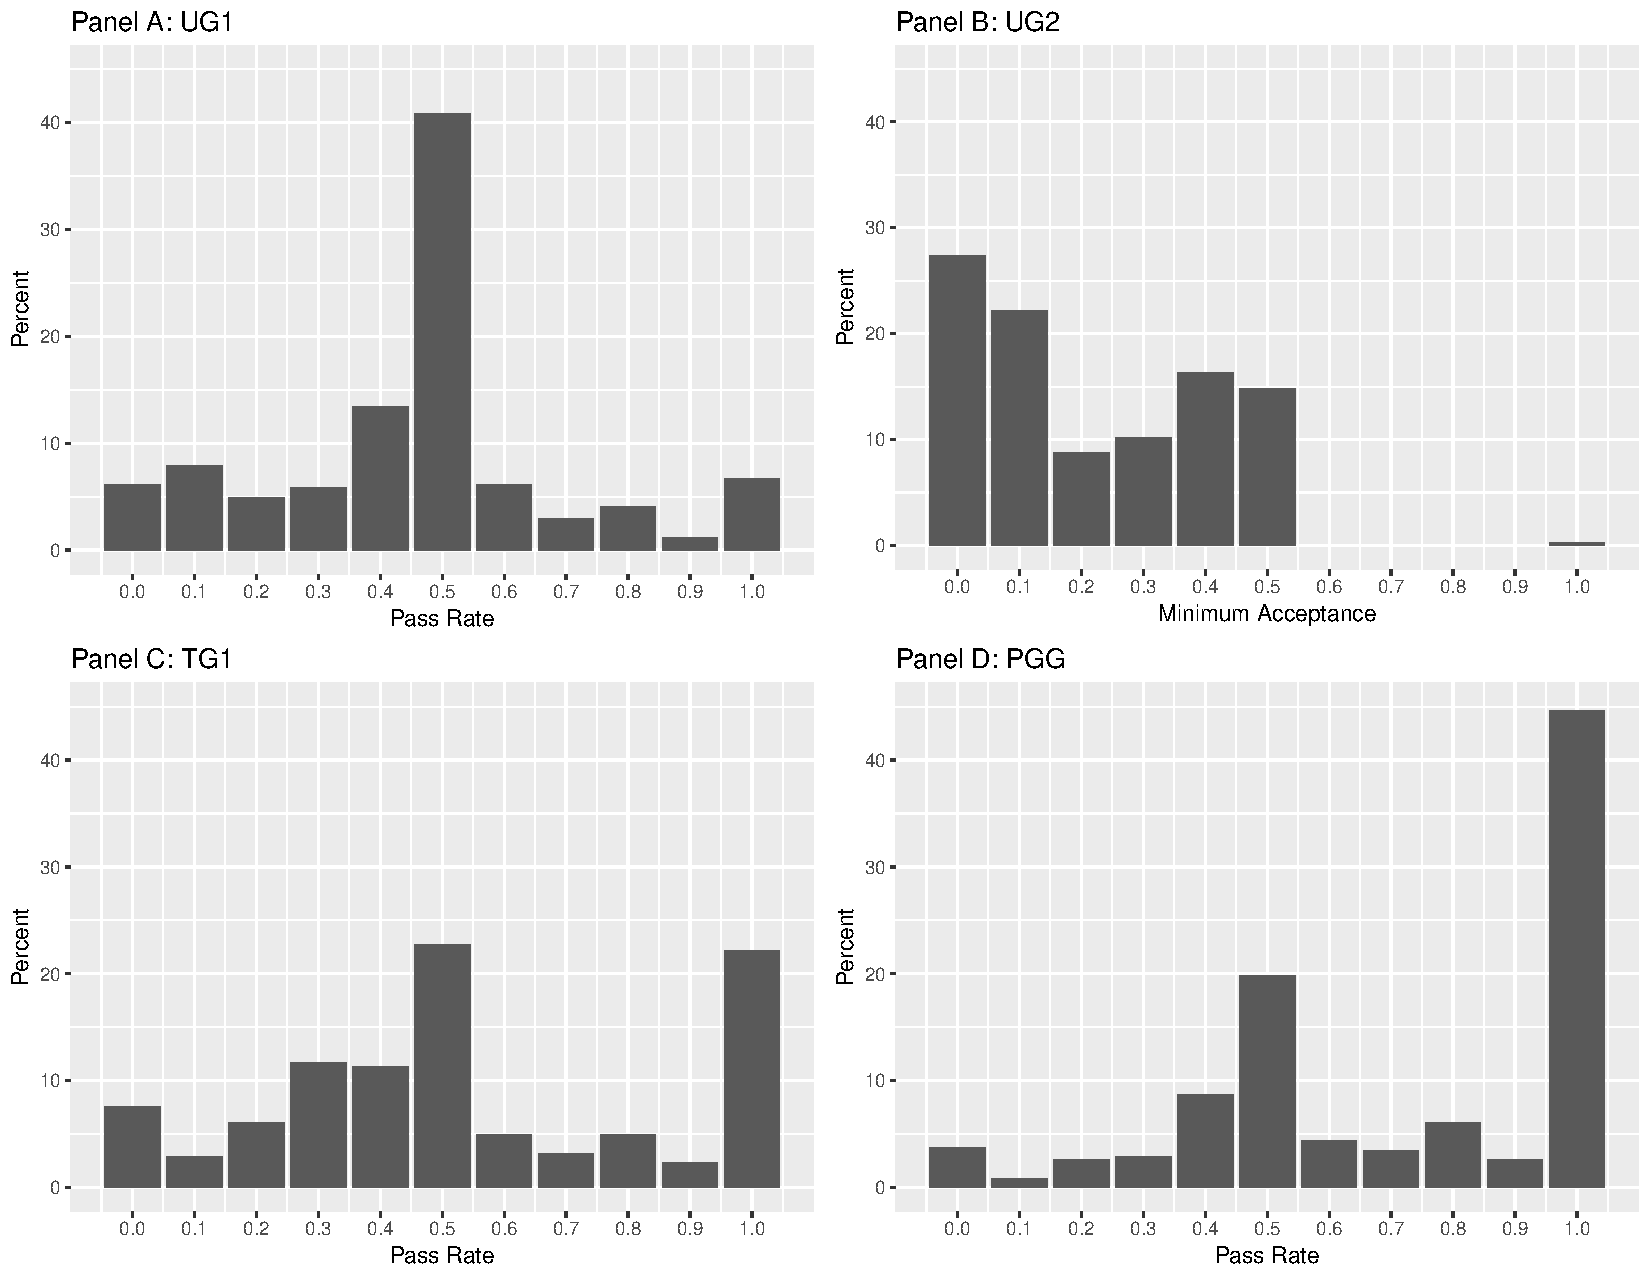
\includegraphics[scale=0.55]{Figure2a.pdf} 
\end{figure}

\begin{figure}[H]
	\centering
	\caption{Distribution of responses in ultimatum, trust, and public goods games}
	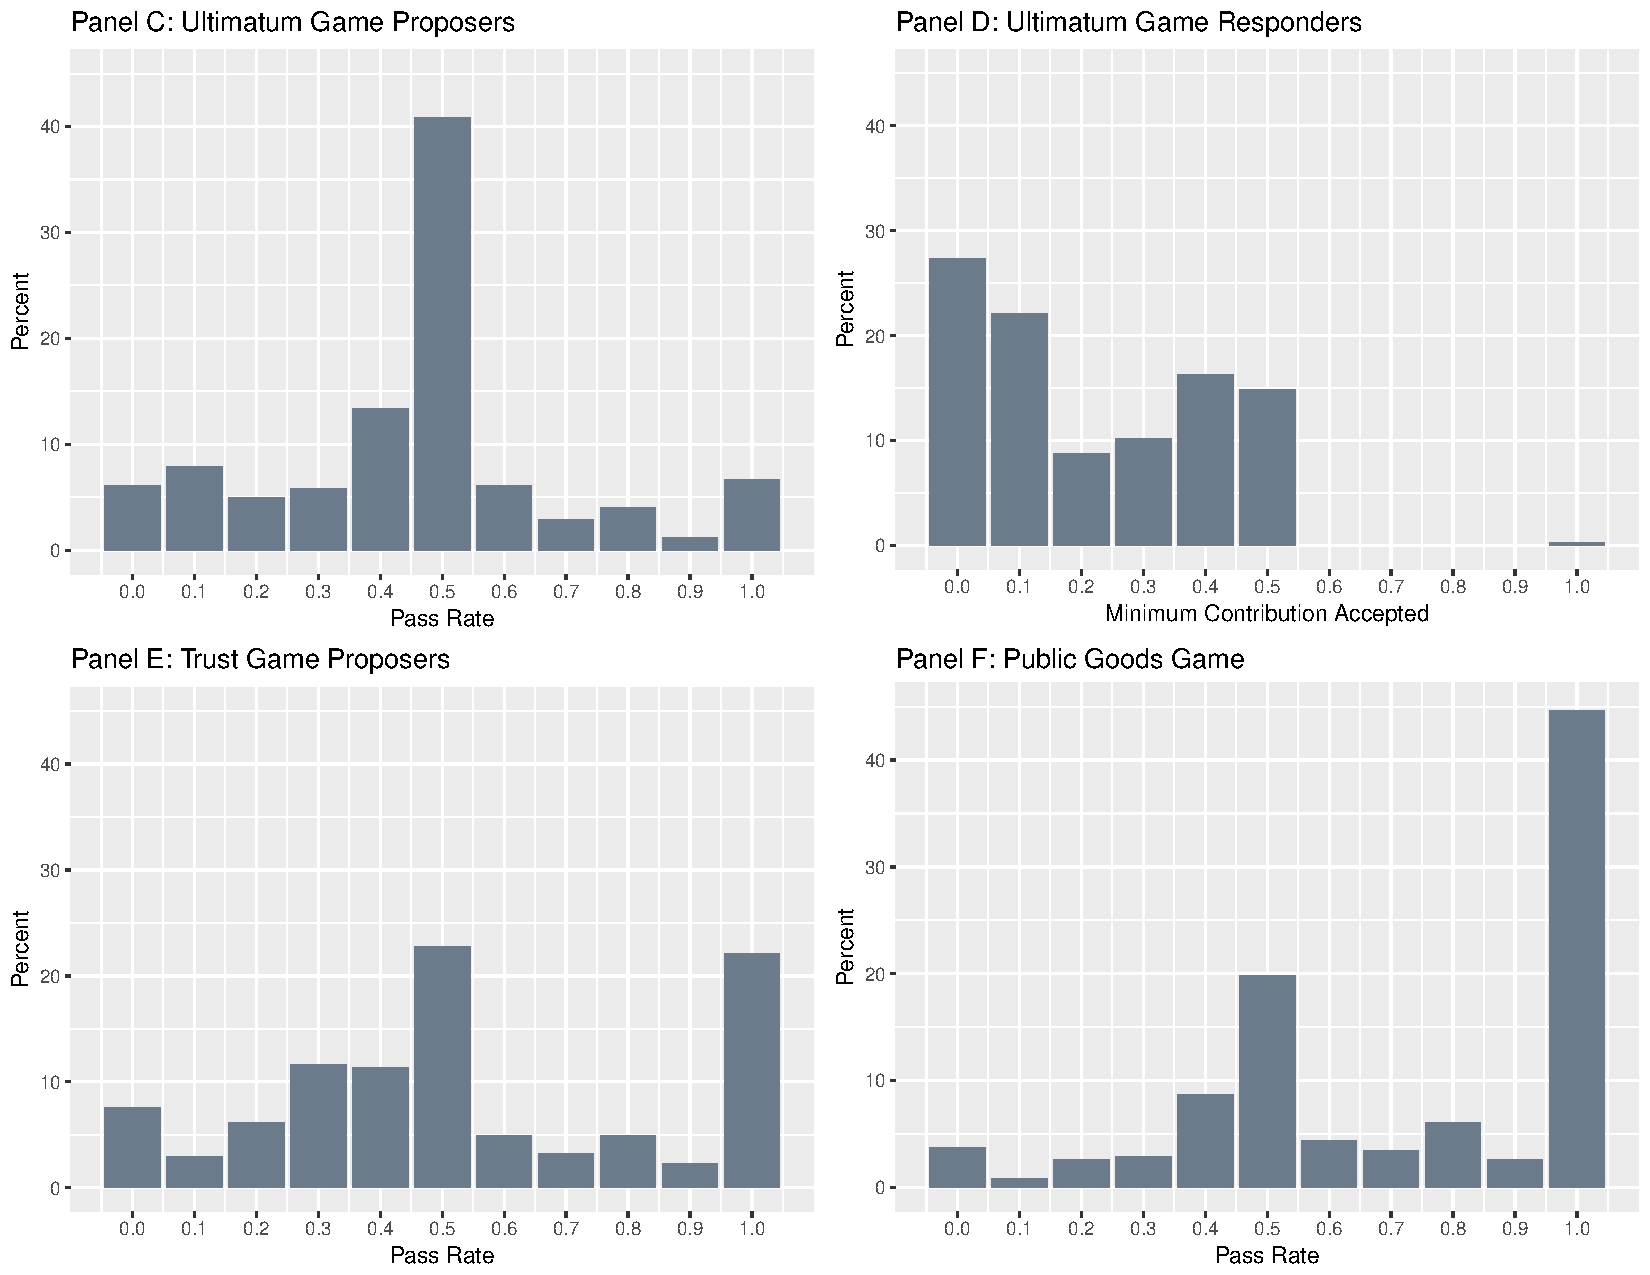
\includegraphics[scale=0.55]{Figure2b.pdf} 
\end{figure}


\begin{figure}[H]
	\centering
	\caption{Distribution of responses from responders in trust game}
	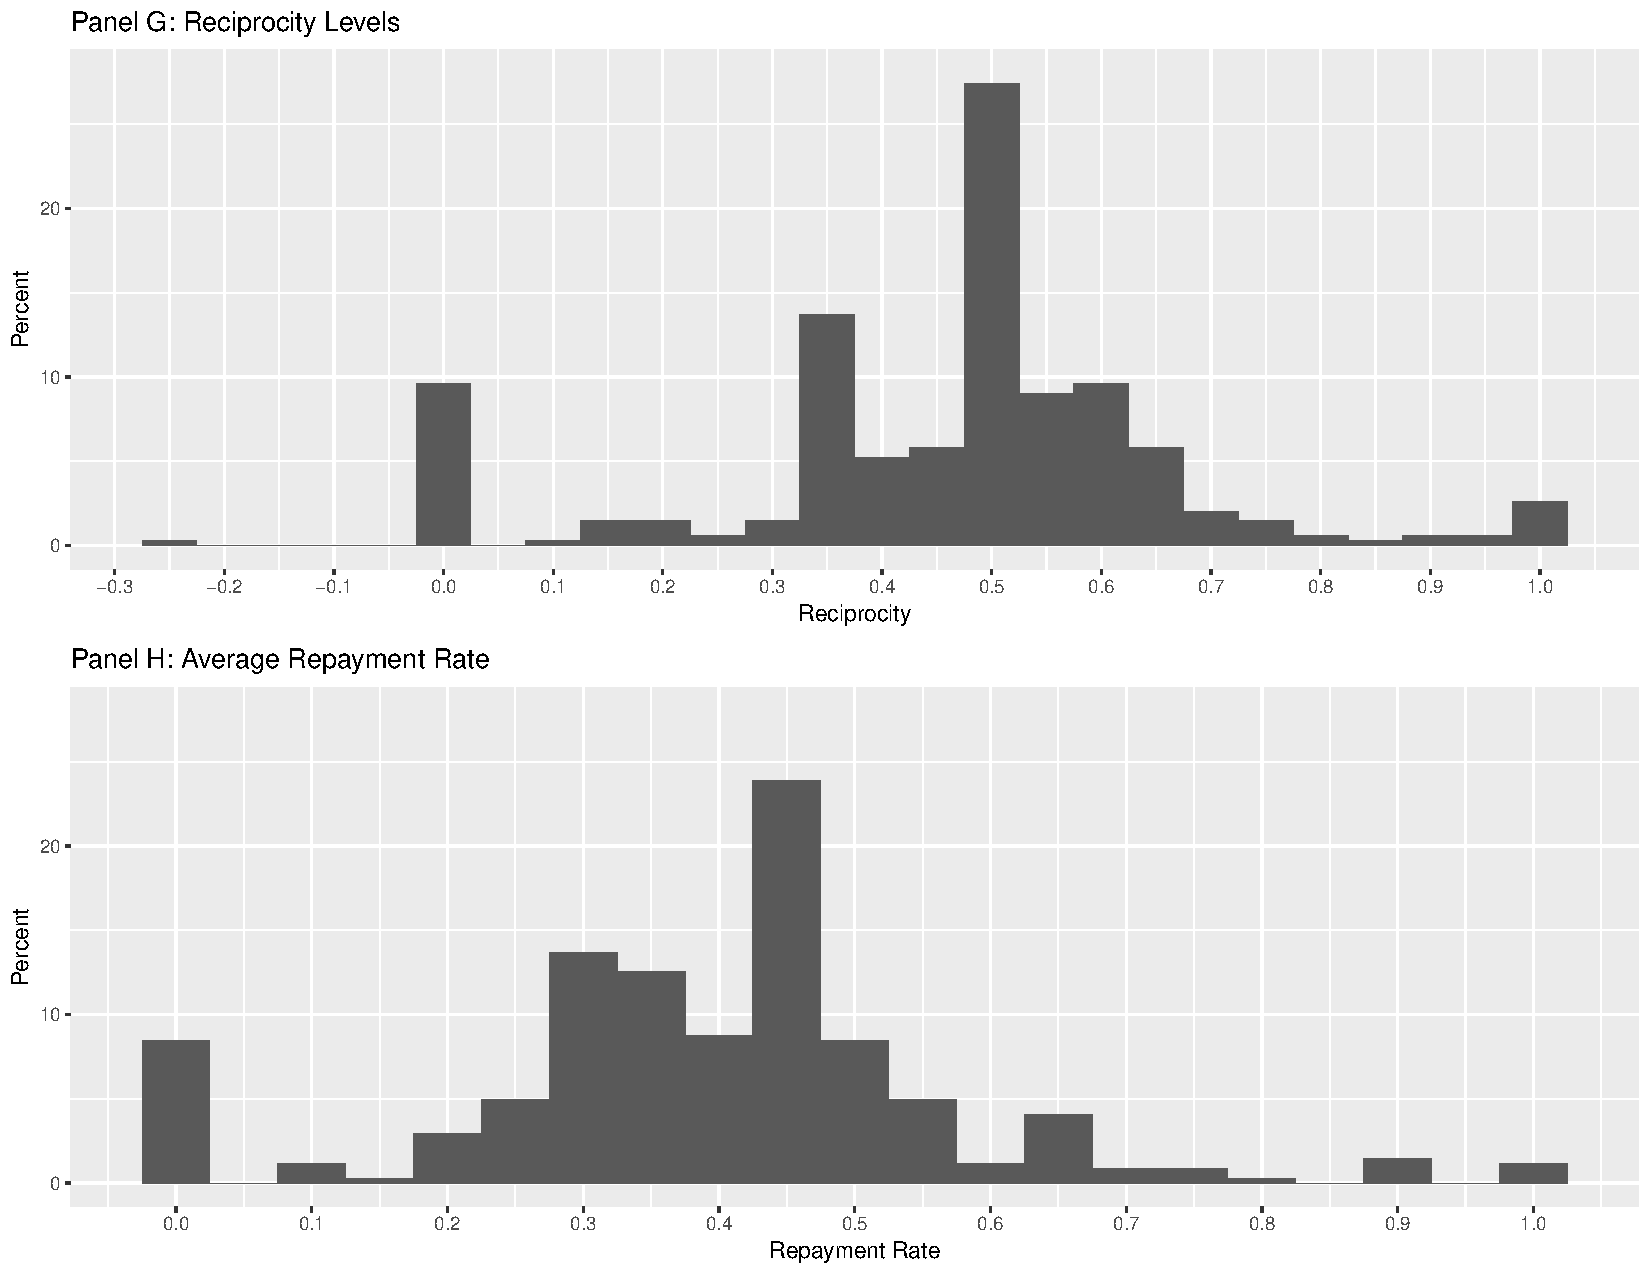
\includegraphics[scale=0.55]{Figure2c.pdf} 
\end{figure}

\begin{figure}[H]
	\centering
	\caption{SRA scores}
	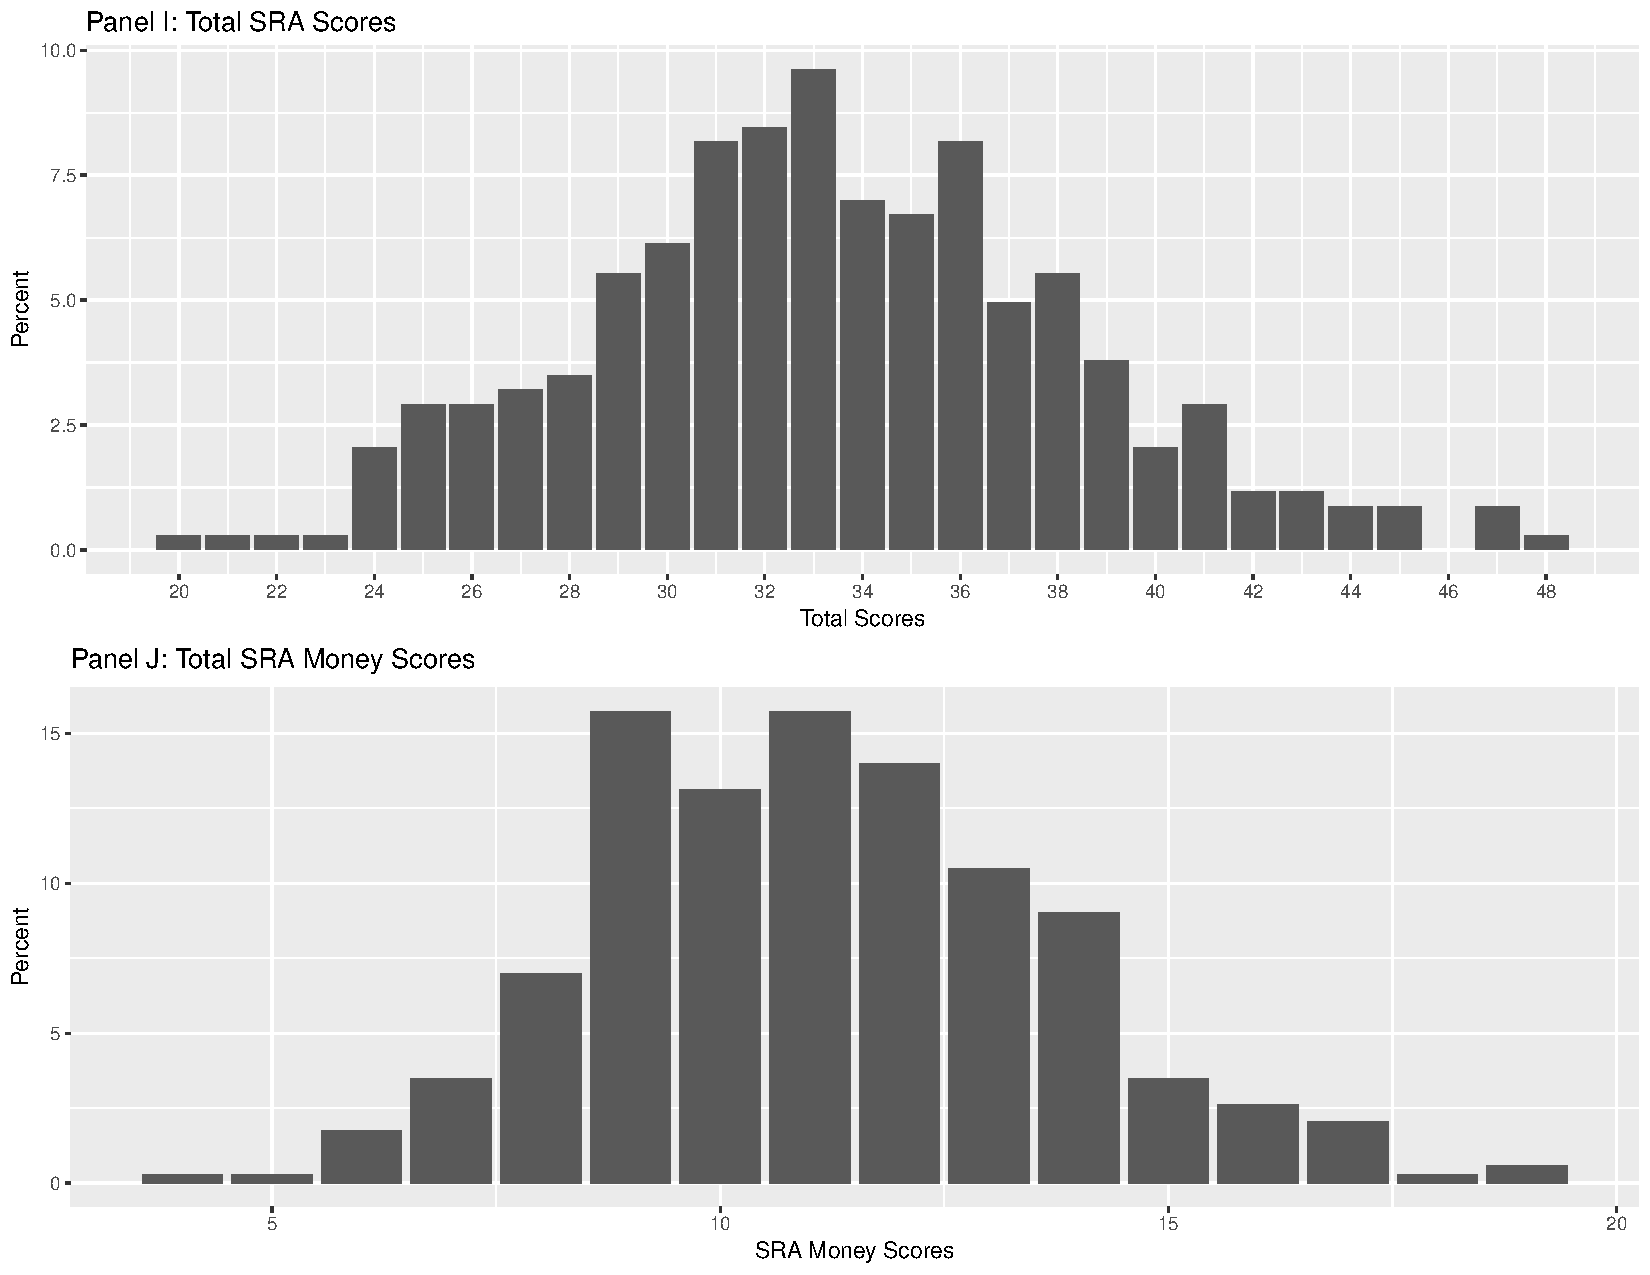
\includegraphics[scale=0.55]{Figure3.pdf} 
\end{figure}

\begin{figure}[H]
	\centering
	\caption{Donations behavior}
	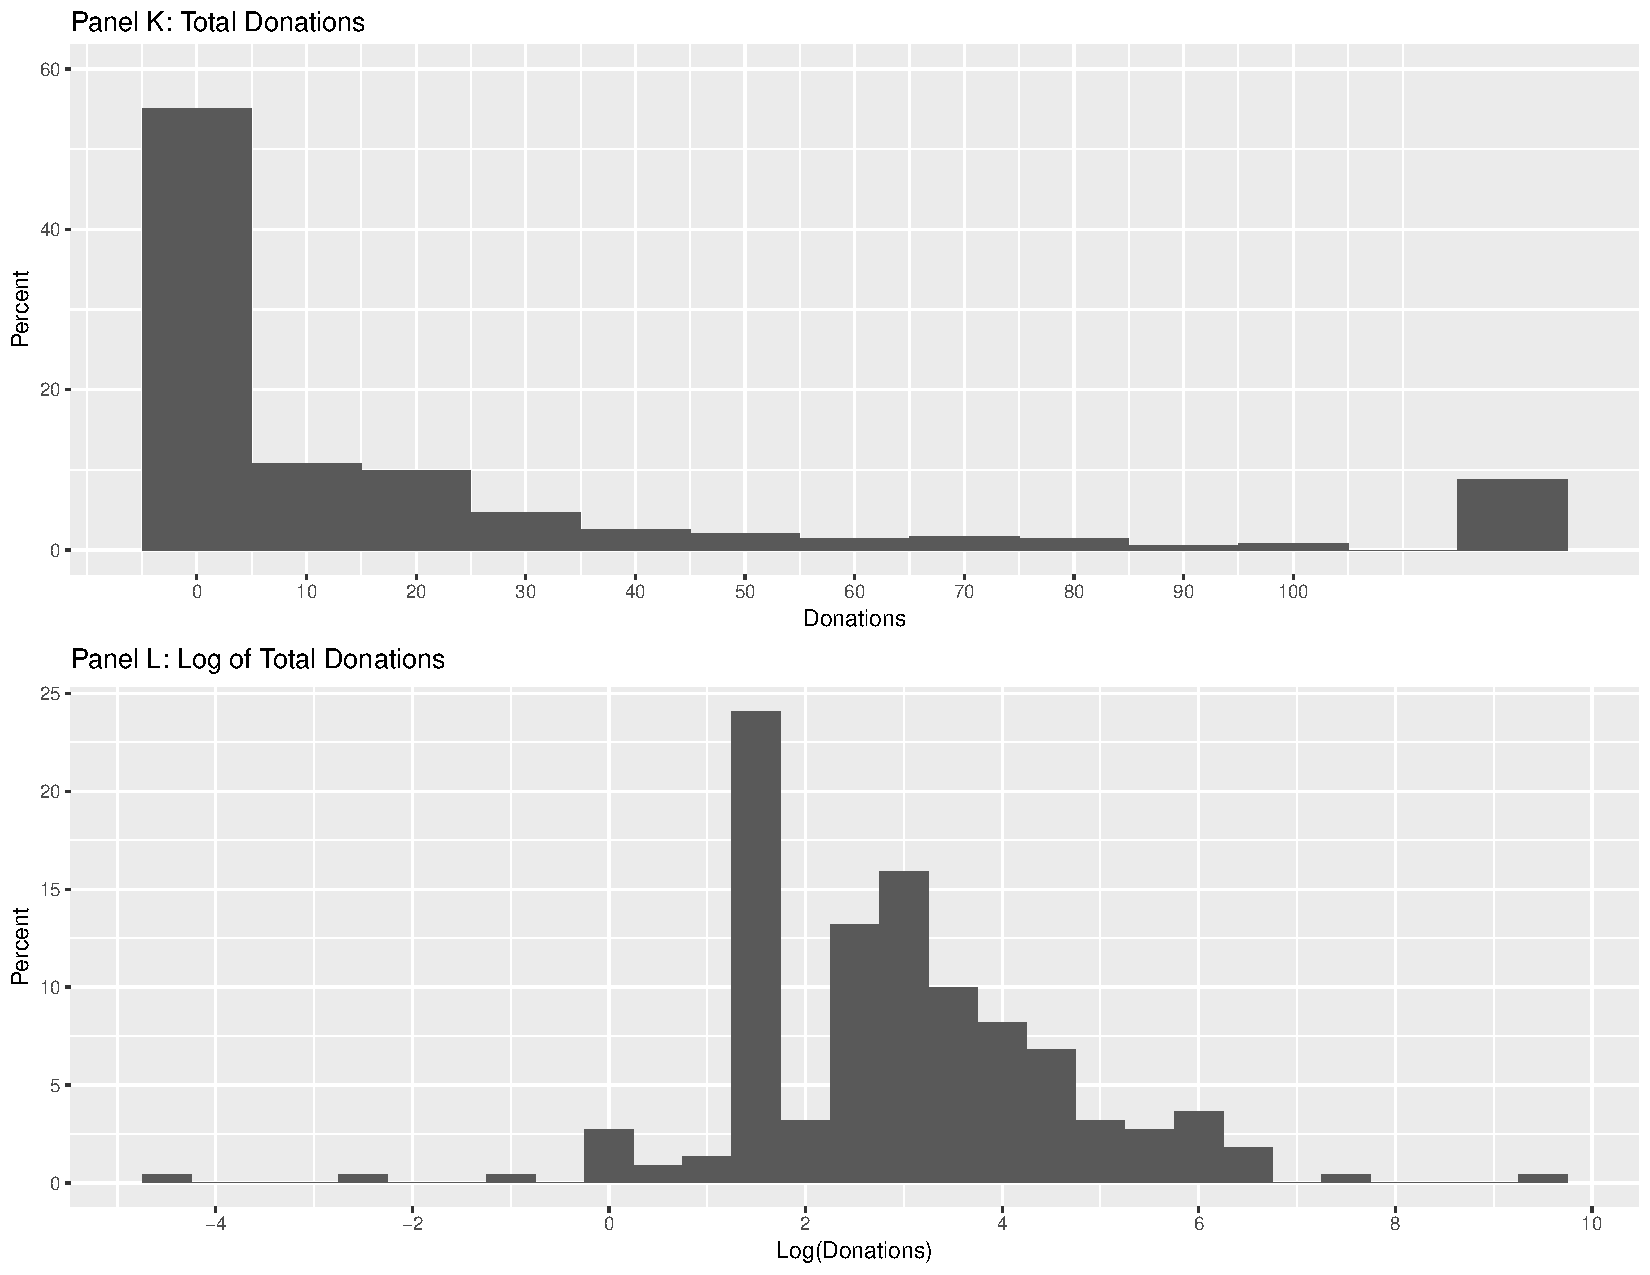
\includegraphics[scale=0.55]{Figure4.pdf} 
\end{figure}

\begin{figure}[H]
	\centering
	\caption{Donations behavior by class year}
	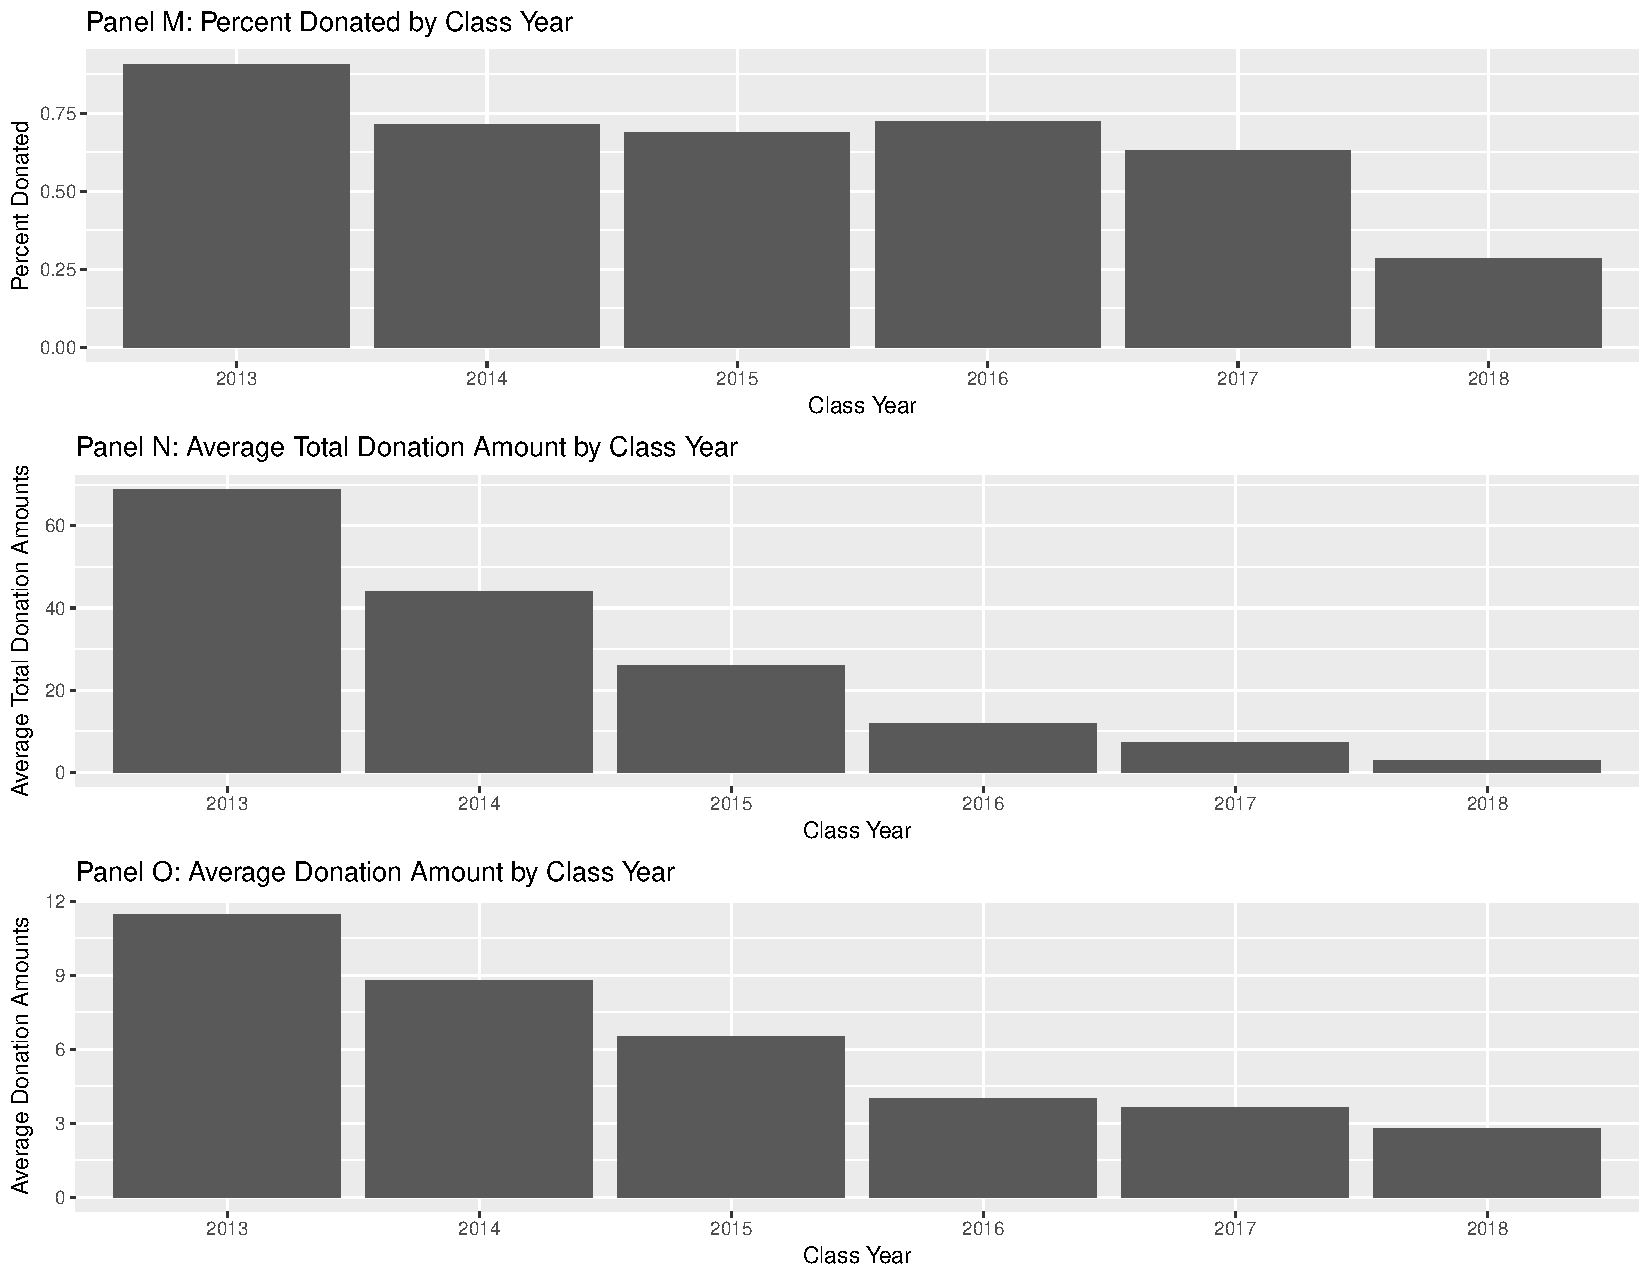
\includegraphics[scale=0.55]{Figure6.pdf} 
\end{figure}

\newpage

%\begin{table}[H] 
%  \caption{Pairwise correlations between game results (Spearman\rq s \(\rho\))} 
%  \label{} \centering
%  \begin{tabular}{rllllll}
%  \hline
% & Alpha &  \ Ultimatum1 & \ Ultimatum2 & \ Trust1 & \ Trust2 & \ Cooperation \\ 
%  \hline
%Alpha &   \ 1.00  & -0.28*** & \ 0.04  & -0.26*** & -0.30*** & -0.16*** \\ 
% Ultimatum1 & -0.28*** & \ 1.00  &  \ 0.09  & \ 0.41*** & \ 0.31*** &  \ 0.30*** \\ 
%  Ultimatum2 &  \ 0.04  &  \ 0.09  &  1.00  & -0.10* & -0.08  & -0.16*** \\ 
%  Trust1 & -0.26*** & \  0.41*** & -0.10* & \ 1.00  & \ 0.45*** &  \ 0.44*** \\ 
%  Trust2 & -0.30*** &  \ 0.31*** & -0.08  &  \ 0.45*** & \ 1.00  &  \ 0.21*** \\ 
%  Cooperation & -0.16*** &  \ 0.30*** & -0.16*** & \  0.44*** & \ 0.21*** &  \ 1.00  \\ 
%   \hline
%      \textit{Note:}  & \multicolumn{6}{r}{$^{*}$p$<$0.1; $^{**}$p$<$0.05; $^{***}$p$<$0.01} \\ 
%      \newline
%\vspace*{1.5 cm}
%\newline
%\end{tabular}
%\end{table}



\begin{table}[H]
  \caption{Pairwise correlations between game results (Spearman\rq s \(\rho\))} 
\label{} \centering
   \begin{adjustbox}{width=\textwidth}
\begin{tabular}{rlllllll}
  \hline
 & Alpha & Rho & Ultimatum1 & Ultimatum2 & Trust1 & Trust2 & \\ 
  \hline
  Rho &  0.54*** &  &  &  &  &  &  \\ 
  Ultimatum1 & -0.28*** & -0.13** &  &  &  &  &  \\ 
  Ultimatum2 &  0.04  & -0.04  &  0.09  &  &  &  &  \\ 
  Trust1 & -0.26*** &  0.04  &  0.41*** & -0.10* &  &  &  \\ 
  Trust2 & -0.30*** & -0.10* &  0.31*** & -0.08  &  0.45*** &  &  \\ 
  Cooperation & -0.16*** & -0.05  &  0.30*** & -0.16*** &  0.44*** &  0.21*** &  \\ 
 \hline
\textit{Note:}  & \multicolumn{6}{r}{$^{*}$p$<$0.1; $^{**}$p$<$0.05; $^{***}$p$<$0.01} \\ 
\newline
\vspace*{1.5 cm}
\newline
\end{tabular}
\end{adjustbox}
\end{table}




\begin{table}[H] \centering 
  \caption{Correlations between game results and SRA scores (Spearman\rq s \(\rho\))} 
  \label{} 
\centering
\begin{tabular}{rlllllllll}
  \hline
 & SRAtotal & SRAmoney \\ 
  \hline
Alpha  & -0.01  & \ \ -0.04  \\ 
  Rho &   -0.03  & \ \ -0.02  \\ 
  Ultimatum1  &  \ 0.02  &  \ \ \ 0.07  \\ 
  Ultimatum2 & -0.05  & \ \ -0.05  \\ 
  Trust1 &  \ 0.07  &  \ \ \ 0.08  \\ 
  Trust2  &  \ 0.04  & \ \ \  0.11** \\ 
  Cooperation  & \  0.06  &  \ \ \ 0.10* \\ 
   \hline
   \textit{Note:}  & \multicolumn{2}{r}{$^{*}$p$<$0.1; $^{**}$p$<$0.05; $^{***}$p$<$0.01} \\ 
\end{tabular}
\end{table}


\begin{table}[H] \centering 
  \caption{Logistic regression models} 
  \label{} 
  \begin{adjustbox}{width=\textwidth}
  \begin{tabular}{@{\extracolsep{5pt}}lcccccccccccc} 
\\[-1.8ex]\hline 
\hline \\[-1.8ex] 
 & \multicolumn{12}{c}{\textit{Dependent variable:}} \\ 
\cline{2-13} 
\\[-1.8ex] & \multicolumn{12}{c}{Donated} \\ 
\\[-1.8ex] & (1) & (2) & (3) & (4) & (5) & (6) & (7) & (8) & (9) & (10) & (11) & (12)\\ 
\hline \\[-1.8ex] 
 Alpha & 0.085 &  &  &  &  &  &  & 0.088 &  &  & 0.084 & 0.088 \\ 
  & (0.080) &  &  &  &  &  &  & (0.104) &  &  & (0.104) & (0.104) \\ 
  & & & & & & & & & & & & \\ 
 Rho &  & 0.004 &  &  &  &  &  & $-$0.0002 &  &  & 0.0001 & $-$0.0002 \\ 
  &  & (0.007) &  &  &  &  &  & (0.008) &  &  & (0.008) & (0.008) \\ 
  & & & & & & & & & & & & \\ 
 Ultimatum1 &  &  & $-$0.060 &  &  &  &  & $-$0.075 &  &  & $-$0.073 & $-$0.076 \\ 
  &  &  & (0.099) &  &  &  &  & (0.116) &  &  & (0.116) & (0.116) \\ 
  & & & & & & & & & & & & \\ 
 Ultimatum2 &  &  &  & 0.119 &  &  &  & 0.132 &  &  & 0.135 & 0.134 \\ 
  &  &  &  & (0.127) &  &  &  & (0.132) &  &  & (0.132) & (0.132) \\ 
  & & & & & & & & & & & & \\ 
 Trust1 &  &  &  &  & 0.001 &  &  & 0.046 &  &  & 0.041 & 0.046 \\ 
  &  &  &  &  & (0.077) &  &  & (0.100) &  &  & (0.101) & (0.100) \\ 
  & & & & & & & & & & & & \\ 
 Trust2 &  &  &  &  &  & 0.005 &  & 0.045 &  &  & 0.044 & 0.040 \\ 
  &  &  &  &  &  & (0.113) &  & (0.131) &  &  & (0.131) & (0.131) \\ 
  & & & & & & & & & & & & \\ 
 Cooperation &  &  &  &  &  &  & $-$0.025 & $-$0.006 &  &  & $-$0.008 & $-$0.009 \\ 
  &  &  &  &  &  &  & (0.081) & (0.092) &  &  & (0.092) & (0.092) \\ 
  & & & & & & & & & & & & \\ 
 SRAtotal &  &  &  &  &  &  &  &  & 0.004 &  & 0.004 &  \\ 
  &  &  &  &  &  &  &  &  & (0.005) &  & (0.005) &  \\ 
  & & & & & & & & & & & & \\ 
 SRAmoney &  &  &  &  &  &  &  &  &  & 0.004 &  & 0.005 \\ 
  &  &  &  &  &  &  &  &  &  & (0.010) &  & (0.010) \\ 
  & & & & & & & & & & & & \\ 
 2017 & 0.342$^{***}$ & 0.338$^{***}$ & 0.339$^{***}$ & 0.336$^{***}$ & 0.337$^{***}$ & 0.337$^{***}$ & 0.339$^{***}$ & 0.343$^{***}$ & 0.332$^{***}$ & 0.335$^{***}$ & 0.339$^{***}$ & 0.342$^{***}$ \\ 
  & (0.080) & (0.080) & (0.080) & (0.080) & (0.080) & (0.080) & (0.080) & (0.081) & (0.080) & (0.080) & (0.081) & (0.081) \\ 
  & & & & & & & & & & & & \\ 
 2016 & 0.431$^{***}$ & 0.431$^{***}$ & 0.432$^{***}$ & 0.426$^{***}$ & 0.429$^{***}$ & 0.429$^{***}$ & 0.430$^{***}$ & 0.435$^{***}$ & 0.425$^{***}$ & 0.426$^{***}$ & 0.430$^{***}$ & 0.431$^{***}$ \\ 
  & (0.076) & (0.077) & (0.077) & (0.076) & (0.077) & (0.077) & (0.077) & (0.078) & (0.077) & (0.077) & (0.078) & (0.078) \\ 
  & & & & & & & & & & & & \\ 
 2015 & 0.401$^{***}$ & 0.393$^{***}$ & 0.397$^{***}$ & 0.390$^{***}$ & 0.393$^{***}$ & 0.393$^{***}$ & 0.393$^{***}$ & 0.405$^{***}$ & 0.389$^{***}$ & 0.388$^{***}$ & 0.401$^{***}$ & 0.399$^{***}$ \\ 
  & (0.084) & (0.083) & (0.084) & (0.083) & (0.083) & (0.083) & (0.083) & (0.085) & (0.083) & (0.084) & (0.085) & (0.085) \\ 
  & & & & & & & & & & & & \\ 
 2014 & 0.424$^{***}$ & 0.421$^{***}$ & 0.423$^{***}$ & 0.416$^{***}$ & 0.420$^{***}$ & 0.420$^{***}$ & 0.422$^{***}$ & 0.417$^{***}$ & 0.416$^{***}$ & 0.416$^{***}$ & 0.414$^{***}$ & 0.414$^{***}$ \\ 
  & (0.083) & (0.083) & (0.083) & (0.083) & (0.083) & (0.083) & (0.083) & (0.084) & (0.083) & (0.083) & (0.084) & (0.084) \\ 
  & & & & & & & & & & & & \\ 
 2013 & 0.619$^{***}$ & 0.621$^{***}$ & 0.622$^{***}$ & 0.619$^{***}$ & 0.618$^{***}$ & 0.618$^{***}$ & 0.621$^{***}$ & 0.623$^{***}$ & 0.614$^{***}$ & 0.613$^{***}$ & 0.620$^{***}$ & 0.618$^{***}$ \\ 
  & (0.080) & (0.080) & (0.080) & (0.080) & (0.080) & (0.080) & (0.081) & (0.082) & (0.080) & (0.081) & (0.082) & (0.082) \\ 
  & & & & & & & & & & & & \\ 
 Female & 0.079 & 0.077 & 0.074 & 0.076 & 0.073 & 0.073 & 0.072 & 0.083 & 0.072 & 0.072 & 0.082 & 0.082 \\ 
  & (0.049) & (0.049) & (0.048) & (0.048) & (0.048) & (0.049) & (0.049) & (0.051) & (0.048) & (0.048) & (0.051) & (0.051) \\ 
  & & & & & & & & & & & & \\ 
 Humanities & $-$0.020 & $-$0.023 & $-$0.022 & $-$0.028 & $-$0.024 & $-$0.024 & $-$0.023 & $-$0.028 & $-$0.019 & $-$0.021 & $-$0.024 & $-$0.026 \\ 
  & (0.063) & (0.063) & (0.063) & (0.064) & (0.064) & (0.064) & (0.064) & (0.064) & (0.064) & (0.064) & (0.065) & (0.065) \\ 
  & & & & & & & & & & & & \\ 
 STEM & 0.022 & 0.025 & 0.025 & 0.024 & 0.027 & 0.027 & 0.027 & 0.016 & 0.027 & 0.029 & 0.017 & 0.018 \\ 
  & (0.055) & (0.055) & (0.055) & (0.055) & (0.055) & (0.055) & (0.055) & (0.056) & (0.055) & (0.055) & (0.056) & (0.056) \\ 
  & & & & & & & & & & & & \\ 
 Constant & 0.197$^{**}$ & 0.250$^{***}$ & 0.272$^{***}$ & 0.224$^{***}$ & 0.246$^{***}$ & 0.245$^{***}$ & 0.264$^{***}$ & 0.161 & 0.113 & 0.199$^{*}$ & 0.032 & 0.113 \\ 
  & (0.078) & (0.062) & (0.075) & (0.067) & (0.074) & (0.079) & (0.083) & (0.130) & (0.170) & (0.119) & (0.201) & (0.161) \\ 
  & & & & & & & & & & & & \\ 
\hline \\[-1.8ex] 
Observations & 343 & 343 & 343 & 343 & 343 & 343 & 343 & 343 & 343 & 343 & 343 & 343 \\ 
Log Likelihood & $-$201.351 & $-$201.760 & $-$201.744 & $-$201.479 & $-$201.929 & $-$201.928 & $-$201.880 & $-$200.578 & $-$201.558 & $-$201.816 & $-$200.201 & $-$200.440 \\ 
Akaike Inf. Crit. & 422.702 & 423.521 & 423.488 & 422.957 & 423.858 & 423.857 & 423.761 & 433.155 & 423.115 & 423.631 & 434.402 & 434.880 \\ 
  Psuedo-R$^{2}$ & 0.14617 & 0.14443 &0.14450 & 0.14563 & 0.14371 &0.14371 & 0.14392 & 0.14947 & 0.14529 & 0.14419 & 0.15108 & 0.15006 \\
  \hline 
\hline \\[-1.8ex] 
\textit{Note:}  & \multicolumn{12}{r}{$^{*}$p$<$0.1; $^{**}$p$<$0.05; $^{***}$p$<$0.01} \\ 
\end{tabular} 
\end{adjustbox}
\end{table} 
  
  
  
 

\newpage

\begin{table}[H] \centering 
  \caption{Linear regression models} 
  \label{} 
   \begin{adjustbox}{width=\textwidth}
   \begin{tabular}{@{\extracolsep{5pt}}lcccccccccccc} 
\\[-1.8ex]\hline 
\hline \\[-1.8ex] 
 & \multicolumn{12}{c}{\textit{Dependent variable:}} \\ 
\cline{2-13} 
\\[-1.8ex] & \multicolumn{12}{c}{Log(Donations)} \\ 
\\[-1.8ex] & (1) & (2) & (3) & (4) & (5) & (6) & (7) & (8) & (9) & (10) & (11) & (12)\\ 
\hline \\[-1.8ex] 
 Alpha & $-$0.152 &  &  &  &  &  &  & 0.035 &  &  & 0.016 & 0.036 \\ 
  & (0.360) &  &  &  &  &  &  & (0.461) &  &  & (0.461) & (0.461) \\ 
  & & & & & & & & & & & & \\ 
 Rho &  & $-$0.041 &  &  &  &  &  & $-$0.041 &  &  & $-$0.038 & $-$0.040 \\ 
  &  & (0.030) &  &  &  &  &  & (0.036) &  &  & (0.036) & (0.036) \\ 
  & & & & & & & & & & & & \\ 
 Ultimatum1 &  &  & 0.226 &  &  &  &  & 0.420 &  &  & 0.446 & 0.425 \\ 
  &  &  & (0.415) &  &  &  &  & (0.463) &  &  & (0.463) & (0.463) \\ 
  & & & & & & & & & & & & \\ 
 Ultimatum2 &  &  &  & $-$0.254 &  &  &  & $-$0.346 &  &  & $-$0.315 & $-$0.330 \\ 
  &  &  &  & (0.548) &  &  &  & (0.557) &  &  & (0.558) & (0.558) \\ 
  & & & & & & & & & & & & \\ 
 Trust1 &  &  &  &  & $-$0.266 &  &  & $-$0.249 &  &  & $-$0.291 & $-$0.254 \\ 
  &  &  &  &  & (0.338) &  &  & (0.435) &  &  & (0.436) & (0.435) \\ 
  & & & & & & & & & & & & \\ 
 Trust2 &  &  &  &  &  & $-$0.889$^{*}$ &  & $-$0.991$^{*}$ &  &  & $-$1.010$^{*}$ & $-$1.022$^{*}$ \\ 
  &  &  &  &  &  & (0.480) &  & (0.563) &  &  & (0.563) & (0.565) \\ 
  & & & & & & & & & & & & \\ 
 Cooperation &  &  &  &  &  &  & 0.489 & 0.534 &  &  & 0.543 & 0.520 \\ 
  &  &  &  &  &  &  & (0.361) & (0.392) &  &  & (0.392) & (0.393) \\ 
  & & & & & & & & & & & & \\ 
 SRAtotal &  &  &  &  &  &  &  &  & 0.020 &  & 0.022 &  \\ 
  &  &  &  &  &  &  &  &  & (0.020) &  & (0.021) &  \\ 
  & & & & & & & & & & & & \\ 
 SRAmoney &  &  &  &  &  &  &  &  &  & 0.028 &  & 0.030 \\ 
  &  &  &  &  &  &  &  &  &  & (0.040) &  & (0.040) \\ 
  & & & & & & & & & & & & \\ 
 2017 & $-$0.637 & $-$0.619 & $-$0.635 & $-$0.600 & $-$0.592 & $-$0.609 & $-$0.671 & $-$0.620 & $-$0.653 & $-$0.645 & $-$0.656 & $-$0.644 \\ 
  & (0.430) & (0.427) & (0.430) & (0.432) & (0.430) & (0.426) & (0.429) & (0.433) & (0.429) & (0.430) & (0.434) & (0.435) \\ 
  & & & & & & & & & & & & \\ 
 2016 & 0.252 & 0.286 & 0.239 & 0.277 & 0.257 & 0.213 & 0.213 & 0.238 & 0.226 & 0.220 & 0.206 & 0.205 \\ 
  & (0.409) & (0.408) & (0.409) & (0.413) & (0.408) & (0.406) & (0.408) & (0.414) & (0.409) & (0.410) & (0.415) & (0.416) \\ 
  & & & & & & & & & & & & \\ 
 2015 & 0.823$^{*}$ & 0.868$^{**}$ & 0.809$^{*}$ & 0.866$^{**}$ & 0.836$^{*}$ & 0.842$^{*}$ & 0.839$^{*}$ & 0.892$^{**}$ & 0.820$^{*}$ & 0.785$^{*}$ & 0.869$^{**}$ & 0.838$^{*}$ \\ 
  & (0.432) & (0.430) & (0.433) & (0.437) & (0.431) & (0.428) & (0.429) & (0.439) & (0.430) & (0.436) & (0.440) & (0.445) \\ 
  & & & & & & & & & & & & \\ 
 2014 & 1.056$^{**}$ & 1.075$^{**}$ & 1.040$^{**}$ & 1.084$^{**}$ & 1.092$^{**}$ & 1.128$^{***}$ & 1.002$^{**}$ & 1.143$^{***}$ & 1.046$^{**}$ & 1.031$^{**}$ & 1.133$^{***}$ & 1.120$^{**}$ \\ 
  & (0.427) & (0.425) & (0.428) & (0.432) & (0.429) & (0.426) & (0.427) & (0.434) & (0.426) & (0.428) & (0.434) & (0.436) \\ 
  & & & & & & & & & & & & \\ 
 2013 & 1.514$^{***}$ & 1.512$^{***}$ & 1.493$^{***}$ & 1.531$^{***}$ & 1.531$^{***}$ & 1.531$^{***}$ & 1.461$^{***}$ & 1.475$^{***}$ & 1.492$^{***}$ & 1.472$^{***}$ & 1.450$^{***}$ & 1.432$^{***}$ \\ 
  & (0.403) & (0.402) & (0.405) & (0.405) & (0.403) & (0.400) & (0.404) & (0.406) & (0.403) & (0.407) & (0.406) & (0.410) \\ 
  & & & & & & & & & & & & \\ 
 Female & $-$0.158 & $-$0.200 & $-$0.142 & $-$0.149 & $-$0.168 & $-$0.079 & $-$0.097 & $-$0.113 & $-$0.146 & $-$0.147 & $-$0.117 & $-$0.117 \\ 
  & (0.215) & (0.215) & (0.211) & (0.212) & (0.214) & (0.212) & (0.213) & (0.227) & (0.211) & (0.211) & (0.227) & (0.228) \\ 
  & & & & & & & & & & & & \\ 
 Humanities & $-$0.386 & $-$0.394 & $-$0.380 & $-$0.376 & $-$0.370 & $-$0.357 & $-$0.399 & $-$0.353 & $-$0.369 & $-$0.368 & $-$0.335 & $-$0.336 \\ 
  & (0.276) & (0.275) & (0.276) & (0.276) & (0.276) & (0.274) & (0.275) & (0.276) & (0.276) & (0.277) & (0.276) & (0.277) \\ 
  & & & & & & & & & & & & \\ 
 STEM & $-$0.449$^{*}$ & $-$0.445$^{*}$ & $-$0.452$^{*}$ & $-$0.446$^{*}$ & $-$0.460$^{*}$ & $-$0.473$^{**}$ & $-$0.419$^{*}$ & $-$0.381 & $-$0.452$^{*}$ & $-$0.444$^{*}$ & $-$0.373 & $-$0.367 \\ 
  & (0.237) & (0.235) & (0.236) & (0.238) & (0.236) & (0.234) & (0.237) & (0.240) & (0.236) & (0.237) & (0.240) & (0.241) \\ 
  & & & & & & & & & & & & \\ 
 Constant & 2.819$^{***}$ & 2.685$^{***}$ & 2.637$^{***}$ & 2.759$^{***}$ & 2.870$^{***}$ & 3.088$^{***}$ & 2.372$^{***}$ & 2.669$^{***}$ & 2.076$^{***}$ & 2.432$^{***}$ & 1.971$^{**}$ & 2.370$^{***}$ \\ 
  & (0.425) & (0.370) & (0.408) & (0.375) & (0.410) & (0.415) & (0.453) & (0.623) & (0.766) & (0.561) & (0.902) & (0.738) \\ 
  & & & & & & & & & & & & \\ 
\hline \\[-1.8ex] 
Observations & 220 & 220 & 220 & 220 & 220 & 220 & 220 & 220 & 220 & 220 & 220 & 220 \\ 
R$^{2}$ & 0.213 & 0.220 & 0.214 & 0.213 & 0.215 & 0.225 & 0.219 & 0.246 & 0.216 & 0.215 & 0.251 & 0.249 \\ 
Adjusted R$^{2}$ & 0.180 & 0.186 & 0.180 & 0.180 & 0.181 & 0.192 & 0.186 & 0.191 & 0.183 & 0.181 & 0.192 & 0.189 \\ 
Residual Std. Error & 1.507 & 1.501 & 1.507  & 1.507  & 1.506  & 1.496  & 1.501  & 1.497  & 1.504  & 1.506  & 1.496  & 1.498 \\ 
& (df = 210) & (df = 210) & (df = 210) & (df = 210) & (df = 210) & (df = 210) & (df = 210) & (df = 204)& (df = 210) & (df = 210) & (df = 203) & (df = 203) \\
F Statistic & 6.327$^{***}$  & 6.570$^{***}$ & 6.344$^{***}$  & 6.332$^{***}$ & 6.389$^{***}$  & 6.786$^{***}$ & 6.561$^{***}$  & 4.449$^{***}$ & 6.437$^{***}$  & 6.373$^{***}$  & 4.245$^{***}$ & 4.198$^{***}$  \\ 
& (df = 9; 210) & (df = 9; 210) & (df = 9; 210) & (df = 9; 210) & (df = 9; 210) & (df = 9; 210) & (df = 9; 210) & (df = 15; 204) & (df = 9; 210) & (df = 9; 210) & (df = 16; 203) & (df = 16; 203) \\
\hline 
\hline \\[-1.8ex] 
\textit{Note:}  & \multicolumn{12}{r}{$^{*}$p$<$0.1; $^{**}$p$<$0.05; $^{***}$p$<$0.01} \\ 
\end{tabular} 
\end{adjustbox}
\end{table}
   
   

   
   

\begin{table}[H] \centering 
  \caption{Best subset logistic regressions} 
  \label{} 
     \begin{adjustbox}{width=\textwidth, totalheight=\textheight-2\baselineskip}
\begin{tabular}{@{\extracolsep{5pt}}lccccc} 
\\[-1.8ex]\hline 
\hline \\[-1.8ex] 
 & \multicolumn{5}{c}{\textit{Dependent variable:}} \\ 
\cline{2-6} 
\\[-1.8ex] & \multicolumn{5}{c}{Donated} \\ 
\\[-1.8ex] & (1) & (2) & (3) & (4) & (5)\\ 
\hline \\[-1.8ex] 
 Alpha & 0.101 & 0.104 &  &  &  \\ 
  & (0.078) & (0.078) &  &  &  \\ 
  & & & & & \\ 
 Ultimatum2 &  &  & 0.100 &  &  \\ 
  &  &  & (0.124) &  &  \\ 
  & & & & & \\ 
 SRA3 & $-$0.097$^{***}$ & $-$0.099$^{***}$ & $-$0.094$^{***}$ & $-$0.096$^{***}$ & $-$0.098$^{***}$ \\ 
  & (0.027) & (0.027) & (0.027) & (0.027) & (0.027) \\ 
  & & & & & \\ 
 SRA4 & 0.099$^{***}$ & 0.097$^{***}$ & 0.097$^{***}$ & 0.097$^{***}$ & 0.096$^{***}$ \\ 
  & (0.029) & (0.029) & (0.029) & (0.029) & (0.029) \\ 
  & & & & & \\ 
 SRA7 &  & 0.015 &  &  & 0.014 \\ 
  &  & (0.020) &  &  & (0.020) \\ 
  & & & & & \\ 
 SRA8 & 0.047 & 0.046 & 0.048 & 0.046 & 0.046 \\ 
  & (0.033) & (0.033) & (0.033) & (0.033) & (0.033) \\ 
  & & & & & \\ 
 SRA10 & $-$0.019 & $-$0.022 & $-$0.018 & $-$0.017 & $-$0.019 \\ 
  & (0.024) & (0.024) & (0.024) & (0.024) & (0.024) \\ 
  & & & & & \\ 
 2017 & 0.326$^{***}$ & 0.329$^{***}$ & 0.318$^{***}$ & 0.320$^{***}$ & 0.322$^{***}$ \\ 
  & (0.078) & (0.078) & (0.078) & (0.078) & (0.078) \\ 
  & & & & & \\ 
 2016 & 0.410$^{***}$ & 0.410$^{***}$ & 0.405$^{***}$ & 0.408$^{***}$ & 0.408$^{***}$ \\ 
  & (0.075) & (0.075) & (0.076) & (0.075) & (0.075) \\ 
  & & & & & \\ 
 2015 & 0.399$^{***}$ & 0.395$^{***}$ & 0.386$^{***}$ & 0.389$^{***}$ & 0.386$^{***}$ \\ 
  & (0.083) & (0.083) & (0.082) & (0.082) & (0.083) \\ 
  & & & & & \\ 
 2014 & 0.405$^{***}$ & 0.403$^{***}$ & 0.398$^{***}$ & 0.401$^{***}$ & 0.399$^{***}$ \\ 
  & (0.081) & (0.081) & (0.081) & (0.081) & (0.081) \\ 
  & & & & & \\ 
 2013 & 0.578$^{***}$ & 0.572$^{***}$ & 0.579$^{***}$ & 0.579$^{***}$ & 0.573$^{***}$ \\ 
  & (0.079) & (0.080) & (0.080) & (0.080) & (0.080) \\ 
  & & & & & \\ 
 Female & 0.036 & 0.032 & 0.032 & 0.030 & 0.026 \\ 
  & (0.049) & (0.050) & (0.049) & (0.049) & (0.049) \\ 
  & & & & & \\ 
 Humanities & $-$0.009 & $-$0.011 & $-$0.017 & $-$0.013 & $-$0.014 \\ 
  & (0.062) & (0.062) & (0.062) & (0.062) & (0.062) \\ 
  & & & & & \\ 
 STEM & 0.037 & 0.038 & 0.040 & 0.043 & 0.043 \\ 
  & (0.054) & (0.054) & (0.054) & (0.054) & (0.054) \\ 
  & & & & & \\ 
 Constant & 0.058 & 0.048 & 0.086 & 0.112 & 0.105 \\ 
  & (0.158) & (0.158) & (0.156) & (0.152) & (0.152) \\ 
  & & & & & \\ 
\hline \\[-1.8ex] 
Observations & 343 & 343 & 343 & 343 & 343 \\ 
Log Likelihood & $-$189.537 & $-$189.223 & $-$190.062 & $-$190.399 & $-$190.142 \\ 
Akaike Inf. Crit. & 407.075 & 408.445 & 408.124 & 406.797 & 408.284 \\ 
Psuedo-R$^{2}$ & 0.19652 & 0.19786 & 0.19428 & 0.19285 & 0.19394 \\
\hline 
\hline \\[-1.8ex] 
\textit{Note:}  & \multicolumn{5}{r}{$^{*}$p$<$0.1; $^{**}$p$<$0.05; $^{***}$p$<$0.01} \\ 
\end{tabular} 
\end{adjustbox}
\end{table} 

  



\begin{table}[H] \centering 
  \caption{Best subset linear regressions} 
  \label{} 
     \begin{adjustbox}{width=\textwidth, totalheight=\textheight-2\baselineskip}
     \begin{tabular}{@{\extracolsep{5pt}}lccccc} 
\\[-1.8ex]\hline 
\hline \\[-1.8ex] 
 & \multicolumn{5}{c}{\textit{Dependent variable:}} \\ 
\cline{2-6} 
\\[-1.8ex] & \multicolumn{5}{c}{Log(Donations)} \\ 
\\[-1.8ex] & (1) & (2) & (3) & (4) & (5)\\ 
\hline \\[-1.8ex] 
 Ultimatum1 & 0.799$^{*}$ & 0.600 & 0.726$^{*}$ & 0.726$^{*}$ & 0.725$^{*}$ \\ 
  & (0.415) & (0.421) & (0.436) & (0.413) & (0.413) \\ 
  & & & & & \\ 
 Ultimatum2 & $-$0.739 &  &  &  &  \\ 
  & (0.527) &  &  &  &  \\ 
  & & & & & \\ 
 Trust1 &  &  & $-$0.450 &  &  \\ 
  &  &  & (0.405) &  &  \\ 
  & & & & & \\ 
 Trust2 & $-$1.476$^{***}$ & $-$1.433$^{***}$ & $-$1.176$^{**}$ & $-$1.395$^{***}$ & $-$1.339$^{***}$ \\ 
  & (0.485) & (0.482) & (0.534) & (0.483) & (0.484) \\ 
  & & & & & \\ 
 Cooperation &  & 0.504 & 0.626$^{*}$ &  &  \\ 
  &  & (0.353) & (0.370) &  &  \\ 
  & & & & & \\ 
 SRA1 &  &  &  &  & $-$0.194 \\ 
  &  &  &  &  & (0.153) \\ 
  & & & & & \\ 
 SRA3 & $-$0.283$^{**}$ & $-$0.272$^{**}$ & $-$0.282$^{**}$ & $-$0.265$^{**}$ & $-$0.242$^{**}$ \\ 
  & (0.115) & (0.114) & (0.115) & (0.115) & (0.116) \\ 
  & & & & & \\ 
 SRA4 & 0.617$^{***}$ & 0.593$^{***}$ & 0.596$^{***}$ & 0.601$^{***}$ & 0.612$^{***}$ \\ 
  & (0.133) & (0.133) & (0.133) & (0.133) & (0.133) \\ 
  & & & & & \\ 
 SRA5 & $-$0.257$^{**}$ & $-$0.237$^{*}$ & $-$0.235$^{*}$ & $-$0.237$^{*}$ & $-$0.204 \\ 
  & (0.128) & (0.127) & (0.127) & (0.128) & (0.130) \\ 
  & & & & & \\ 
 SRA6 & 0.231$^{*}$ & 0.231$^{*}$ & 0.248$^{*}$ & 0.221 & 0.263$^{*}$ \\ 
  & (0.136) & (0.136) & (0.137) & (0.136) & (0.140) \\ 
  & & & & & \\ 
 2017 & $-$0.481 & $-$0.590 & $-$0.556 & $-$0.553 & $-$0.503 \\ 
  & (0.411) & (0.409) & (0.410) & (0.409) & (0.410) \\ 
  & & & & & \\ 
 2016 & 0.244 & 0.134 & 0.149 & 0.161 & 0.208 \\ 
  & (0.394) & (0.390) & (0.390) & (0.390) & (0.391) \\ 
  & & & & & \\ 
 2015 & 0.909$^{**}$ & 0.838$^{**}$ & 0.840$^{**}$ & 0.809$^{*}$ & 0.820$^{*}$ \\ 
  & (0.424) & (0.419) & (0.418) & (0.419) & (0.419) \\ 
  & & & & & \\ 
 2014 & 1.097$^{***}$ & 0.973$^{**}$ & 0.995$^{**}$ & 1.011$^{**}$ & 1.061$^{**}$ \\ 
  & (0.412) & (0.409) & (0.409) & (0.409) & (0.410) \\ 
  & & & & & \\ 
 2013 & 1.406$^{***}$ & 1.324$^{***}$ & 1.328$^{***}$ & 1.359$^{***}$ & 1.395$^{***}$ \\ 
  & (0.391) & (0.390) & (0.390) & (0.390) & (0.391) \\ 
  & & & & & \\ 
 Female & $-$0.080 & $-$0.019 & $-$0.073 & $-$0.067 & $-$0.113 \\ 
  & (0.209) & (0.212) & (0.217) & (0.209) & (0.212) \\ 
  & & & & & \\ 
 Humanities & $-$0.304 & $-$0.344 & $-$0.331 & $-$0.324 & $-$0.296 \\ 
  & (0.262) & (0.262) & (0.263) & (0.263) & (0.263) \\ 
  & & & & & \\ 
 STEM & $-$0.264 & $-$0.275 & $-$0.254 & $-$0.312 & $-$0.279 \\ 
  & (0.228) & (0.227) & (0.228) & (0.226) & (0.227) \\ 
  & & & & & \\ 
 Constant & 1.660$^{**}$ & 1.255 & 1.179 & 1.554$^{*}$ & 1.753$^{**}$ \\ 
  & (0.838) & (0.860) & (0.862) & (0.836) & (0.849) \\ 
  & & & & & \\ 
\hline \\[-1.8ex] 
Observations & 220 & 220 & 220 & 220 & 220 \\ 
R$^{2}$ & 0.325 & 0.325 & 0.329 & 0.318 & 0.324 \\ 
Adjusted R$^{2}$ & 0.275 & 0.275 & 0.276 & 0.272 & 0.274 \\ 
Residual Std. Error & 1.417 (df = 204) & 1.416 (df = 204) & 1.416 (df = 203) & 1.420 (df = 205) & 1.418 (df = 204) \\ 
&  (df = 204) &  (df = 204) &  (df = 203) &  (df = 205) &  (df = 204) \\
F Statistic & 6.544$^{***}$  & 6.551$^{***}$  & 6.227$^{***}$  & 6.839$^{***}$  & 6.510$^{***}$  \\ 
&  (df = 15; 204) &  (df = 15; 204) &  (df = 16; 203) &  (df = 14; 205) &  (df = 15; 204) \\
\hline 
\hline \\[-1.8ex] 
\textit{Note:}  & \multicolumn{5}{r}{$^{*}$p$<$0.1; $^{**}$p$<$0.05; $^{***}$p$<$0.01} \\ 
\end{tabular} 
\end{adjustbox}
\end{table} 
     

  

\begin{table}[H] \centering 
  \caption{Logistic predictive models on 2013-2016 alumni} 
  \label{} 
  \begin{adjustbox}{width=\textwidth}
\begin{tabular}{@{\extracolsep{5pt}}lcccccccccccc} 
\\[-1.8ex]\hline 
\hline \\[-1.8ex] 
 & \multicolumn{12}{c}{\textit{Dependent variable:}} \\ 
\cline{2-13} 
\\[-1.8ex] & \multicolumn{12}{c}{Donated} \\ 
\\[-1.8ex] & (1) & (2) & (3) & (4) & (5) & (6) & (7) & (8) & (9) & (10) & (11) & (12)\\ 
\hline \\[-1.8ex] 
 Alpha & 0.212$^{**}$ &  &  &  &  &  &  & 0.214$^{*}$ &  &  & 0.218$^{*}$ & 0.222$^{*}$ \\ 
  & (0.094) &  &  &  &  &  &  & (0.119) &  &  & (0.119) & (0.119) \\ 
  & & & & & & & & & & & & \\ 
 Rho &  & 0.011 &  &  &  &  &  & 0.003 &  &  & 0.003 & 0.003 \\ 
  &  & (0.008) &  &  &  &  &  & (0.010) &  &  & (0.010) & (0.010) \\ 
  & & & & & & & & & & & & \\ 
 Ultimatum1 &  &  & $-$0.049 &  &  &  &  & $-$0.054 &  &  & $-$0.054 & $-$0.059 \\ 
  &  &  & (0.121) &  &  &  &  & (0.138) &  &  & (0.138) & (0.138) \\ 
  & & & & & & & & & & & & \\ 
 Ultimatum2 &  &  &  & 0.276$^{*}$ &  &  &  & 0.291$^{*}$ &  &  & 0.301$^{*}$ & 0.308$^{**}$ \\ 
  &  &  &  & (0.150) &  &  &  & (0.154) &  &  & (0.154) & (0.154) \\ 
  & & & & & & & & & & & & \\ 
 Trust1 &  &  &  &  & $-$0.033 &  &  & $-$0.008 &  &  & $-$0.016 & $-$0.005 \\ 
  &  &  &  &  & (0.093) &  &  & (0.116) &  &  & (0.116) & (0.116) \\ 
  & & & & & & & & & & & & \\ 
 Trust2 &  &  &  &  &  & 0.028 &  & 0.160 &  &  & 0.172 & 0.161 \\ 
  &  &  &  &  &  & (0.129) &  & (0.151) &  &  & (0.152) & (0.151) \\ 
  & & & & & & & & & & & & \\ 
 Cooperation &  &  &  &  &  &  & $-$0.037 & 0.005 &  &  & 0.001 & $-$0.007 \\ 
  &  &  &  &  &  &  & (0.099) & (0.109) &  &  & (0.109) & (0.109) \\ 
  & & & & & & & & & & & & \\ 
 SRAtotal &  &  &  &  &  &  &  &  & 0.003 &  & 0.005 &  \\ 
  &  &  &  &  &  &  &  &  & (0.006) &  & (0.006) &  \\ 
  & & & & & & & & & & & & \\ 
 SRAmoney &  &  &  &  &  &  &  &  &  & 0.011 &  & 0.016 \\ 
  &  &  &  &  &  &  &  &  &  & (0.012) &  & (0.012) \\ 
  & & & & & & & & & & & & \\ 
 Constant & 0.650$^{***}$ & 0.776$^{***}$ & 0.783$^{***}$ & 0.699$^{***}$ & 0.777$^{***}$ & 0.746$^{***}$ & 0.786$^{***}$ & 0.543$^{***}$ & 0.662$^{***}$ & 0.635$^{***}$ & 0.359 & 0.367$^{*}$ \\ 
  & (0.056) & (0.032) & (0.064) & (0.044) & (0.058) & (0.066) & (0.077) & (0.138) & (0.199) & (0.140) & (0.243) & (0.194) \\ 
  & & & & & & & & & & & & \\ 
\hline \\[-1.8ex] 
Observations & 216 & 216 & 216 & 216 & 216 & 216 & 216 & 216 & 216 & 216 & 216 & 216 \\ 
Log Likelihood & $-$121.414 & $-$123.035 & $-$123.866 & $-$122.244 & $-$123.885 & $-$123.927 & $-$123.879 & $-$119.047 & $-$123.827 & $-$123.536 & $-$118.605 & $-$118.183 \\ 
Akaike Inf. Crit. & 246.828 & 250.069 & 251.733 & 248.488 & 251.770 & 251.853 & 251.758 & 254.095 & 251.655 & 251.072 & 255.211 & 254.365 \\ 
MSPE & 0.26410 & 0.25548 & 0.24911 & 0.24984 & 0.24999 & 0.24837 & 0.24903 & 0.26641 & 0.24726 & 0.24649 & 0.26513 & 0.26493 \\
\hline 
\hline \\[-1.8ex] 
\textit{Note:}  & \multicolumn{12}{r}{$^{*}$p$<$0.1; $^{**}$p$<$0.05; $^{***}$p$<$0.01} \\ 
\end{tabular} 
\end{adjustbox}
\end{table} 

\begin{table}[H] \centering 
  \caption{Best subsets logistic predictive models on 2013-2016 alumni} 
  \label{} 
  \begin{adjustbox}{width=\textwidth}
\begin{tabular}{@{\extracolsep{5pt}}lccccc} 
\\[-1.8ex]\hline 
\hline \\[-1.8ex] 
 & \multicolumn{5}{c}{\textit{Dependent variable:}} \\ 
\cline{2-6} 
\\[-1.8ex] & \multicolumn{5}{c}{Donated} \\ 
\\[-1.8ex] & (1) & (2) & (3) & (4) & (5)\\ 
\hline \\[-1.8ex] 
 Alpha & 0.283$^{***}$ & 0.281$^{***}$ & 0.244$^{***}$ & 0.246$^{***}$ & 0.249$^{***}$ \\ 
  & (0.093) & (0.094) & (0.090) & (0.089) & (0.090) \\ 
  & & & & & \\ 
 Average Return & 0.203 & 0.177 &  &  &  \\ 
  & (0.151) & (0.151) &  &  &  \\ 
  & & & & & \\ 
 Ultimatum2 & 0.225 &  & 0.208 & 0.203 &  \\ 
  & (0.144) &  & (0.143) & (0.143) &  \\ 
  & & & & & \\ 
 SRA3 & $-$0.086$^{***}$ & $-$0.094$^{***}$ & $-$0.091$^{***}$ & $-$0.091$^{***}$ & $-$0.098$^{***}$ \\ 
  & (0.032) & (0.031) & (0.031) & (0.031) & (0.031) \\ 
  & & & & & \\ 
 SRA4 & 0.137$^{***}$ & 0.140$^{***}$ & 0.143$^{***}$ & 0.139$^{***}$ & 0.141$^{***}$ \\ 
  & (0.032) & (0.032) & (0.033) & (0.032) & (0.032) \\ 
  & & & & & \\ 
 SR10 &  &  & $-$0.022 &  &  \\ 
  &  &  & (0.025) &  &  \\ 
  & & & & & \\ 
 Constant & 0.284$^{*}$ & 0.361$^{**}$ & 0.450$^{***}$ & 0.399$^{***}$ & 0.455$^{***}$ \\ 
  & (0.170) & (0.163) & (0.158) & (0.147) & (0.142) \\ 
  & & & & & \\ 
\hline \\[-1.8ex] 
Observations & 216 & 216 & 216 & 216 & 216 \\ 
Log Likelihood & $-$107.722 & $-$108.970 & $-$108.264 & $-$108.649 & $-$109.672 \\ 
Akaike Inf. Crit. & 227.444 & 227.940 & 228.528 & 227.298 & 227.345 \\ 
MSPE & 0.26557 & 0.26473 & 0.26193 & 0.26468 & 0.26419 \\
\hline 
\hline \\[-1.8ex] 
\textit{Note:}  & \multicolumn{5}{r}{$^{*}$p$<$0.1; $^{**}$p$<$0.05; $^{***}$p$<$0.01} \\ 
\end{tabular} 
\end{adjustbox}
\end{table} 

\begin{table}[H] \centering 
  \caption{Lasso penalized logistic predictive model on 2013-2016 alumni} 
  \label{} 
\begin{tabular}{@{\extracolsep{5pt}}lc} 
\\[-1.8ex]\hline 
\hline \\[-1.8ex] 
 & \multicolumn{1}{c}{\textit{Dependent variable:}} \\ 
\cline{2-2} 
\\[-1.8ex] & Donated \\ 
\hline \\[-1.8ex] 
 Alpha & 0.13728 \\ 
  & \\ 
 Ultimatum2 & 0.07993 \\ 
  & \\ 
 SRA3 & $-$0.05163$^{*}$ \\ 
  & \\ 
 SRA4 & 0.09403$^{***}$ \\ 
  & \\ 
 Constant & 0.51105 \\ 
  & \\ 
\hline \\[-1.8ex] 
Observations & 216 \\ 
MSPE & 0.25177 \\
\hline 
\hline \\[-1.8ex] 
\textit{Note:}  & \multicolumn{1}{r}{$^{*}$p$<$0.1; $^{**}$p$<$0.05; $^{***}$p$<$0.01} \\ 
\end{tabular} 
\end{table} 

\newpage

\begin{table}[H] \centering 
  \caption{Linear predictive models on 2013-2016 alumni} 
  \label{} 
  \begin{adjustbox}{width=\textwidth}
  \begin{tabular}{@{\extracolsep{5pt}}lcccccccccccc} 
\\[-1.8ex]\hline 
\hline \\[-1.8ex] 
 & \multicolumn{12}{c}{\textit{Dependent variable:}} \\ 
\cline{2-13} 
\\[-1.8ex] & \multicolumn{12}{c}{Log(Donations)} \\ 
\\[-1.8ex] & (1) & (2) & (3) & (4) & (5) & (6) & (7) & (8) & (9) & (10) & (11) & (12)\\ 
\hline \\[-1.8ex] 
 Alpha & $-$0.279 &  &  &  &  &  &  & 0.170 &  &  & 0.192 & 0.250 \\ 
  & (0.401) &  &  &  &  &  &  & (0.488) &  &  & (0.488) & (0.487) \\ 
  & & & & & & & & & & & & \\ 
 Rho &  & $-$0.060$^{*}$ &  &  &  &  &  & $-$0.070$^{*}$ &  &  & $-$0.066 & $-$0.068$^{*}$ \\ 
  &  & (0.034) &  &  &  &  &  & (0.040) &  &  & (0.040) & (0.040) \\ 
  & & & & & & & & & & & & \\ 
 Ultimatum1 &  &  & 0.603 &  &  &  &  & 0.486 &  &  & 0.487 & 0.456 \\ 
  &  &  & (0.476) &  &  &  &  & (0.523) &  &  & (0.523) & (0.520) \\ 
  & & & & & & & & & & & & \\ 
 Ultimatum2 &  &  &  & 0.134 &  &  &  & 0.017 &  &  & 0.083 & 0.128 \\ 
  &  &  &  & (0.608) &  &  &  & (0.612) &  &  & (0.616) & (0.612) \\ 
  & & & & & & & & & & & & \\ 
 Trust1 &  &  &  &  & 0.195 &  &  & 0.120 &  &  & 0.070 & 0.121 \\ 
  &  &  &  &  & (0.388) &  &  & (0.468) &  &  & (0.471) & (0.465) \\ 
  & & & & & & & & & & & & \\ 
 Trust2 &  &  &  &  &  & $-$0.526 &  & $-$0.978 &  &  & $-$0.939 & $-$0.979 \\ 
  &  &  &  &  &  & (0.528) &  & (0.607) &  &  & (0.608) & (0.603) \\ 
  & & & & & & & & & & & & \\ 
 Cooperation &  &  &  &  &  &  & 1.015$^{**}$ & 0.964$^{**}$ &  &  & 0.974$^{**}$ & 0.925$^{**}$ \\ 
  &  &  &  &  &  &  & (0.402) & (0.429) &  &  & (0.429) & (0.427) \\ 
  & & & & & & & & & & & & \\ 
 SRAtotal &  &  &  &  &  &  &  &  & 0.030 &  & 0.024 &  \\ 
  &  &  &  &  &  &  &  &  & (0.024) &  & (0.024) &  \\ 
  & & & & & & & & & & & & \\ 
 SRAmoney &  &  &  &  &  &  &  &  &  & 0.093$^{*}$ &  & 0.083$^{*}$ \\ 
  &  &  &  &  &  &  &  &  &  & (0.048) &  & (0.048) \\ 
  & & & & & & & & & & & & \\ 
 Constant & 3.426$^{***}$ & 3.194$^{***}$ & 2.991$^{***}$ & 3.244$^{***}$ & 3.169$^{***}$ & 3.516$^{***}$ & 2.542$^{***}$ & 2.544$^{***}$ & 2.258$^{***}$ & 2.203$^{***}$ & 1.712$^{*}$ & 1.569$^{*}$ \\ 
  & (0.248) & (0.126) & (0.253) & (0.184) & (0.241) & (0.270) & (0.313) & (0.581) & (0.822) & (0.563) & (1.022) & (0.810) \\ 
  & & & & & & & & & & & & \\ 
\hline \\[-1.8ex] 
Observations & 164 & 164 & 164 & 164 & 164 & 164 & 164 & 164 & 164 & 164 & 164 & 164 \\ 
R$^{2}$ & 0.003 & 0.019 & 0.010 & 0.0003 & 0.002 & 0.006 & 0.038 & 0.076 & 0.010 & 0.023 & 0.082 & 0.093 \\ 
Adjusted R$^{2}$ & $-$0.003 & 0.013 & 0.004 & $-$0.006 & $-$0.005 & $-$0.00005 & 0.032 & 0.035 & 0.003 & 0.017 & 0.034 & 0.047 \\ 
Resid Std. Error & 1.513 & 1.501 & 1.508 & 1.515  & 1.514 & 1.510 & 1.486  & 1.484 & 1.508 & 1.498 & 1.484  & 1.475\\ 
& (df = 162) & (df = 162) & (df = 162) & (df = 162) & (df = 162) & (df = 162) & (df = 162) & (df = 156) & (df = 162) & (df = 162) & (df = 155) & (df = 155) \\
F Statistic & 0.484  & 3.073$^{*}$  & 1.608  & 0.049  & 0.254 & 0.992  & 6.380$^{**}$  & 1.834$^{*}$  & 1.559  & 3.790$^{*}$ & 1.727$^{*}$  & 1.994$^{*}$  \\ 
& (df = 1; 162) & (df = 1; 162) & (df = 1; 162) & (df = 1; 162) & (df = 1; 162) & (df = 1; 162) & (df = 1; 162) & (df = 7; 156) & (df = 1; 162) & (df = 1; 162)  & (df = 8; 155) & (df = 8; 155) \\
RMSE & 2.34232 & 2.33714 & 2.32946  & 2.32775 & 2.34274 & 2.31619 & 2.41094 & 2.41697 & 2.33212 & 2.33100 & 2.41228 & 2.40812 \\
\hline 
\hline \\[-1.8ex] 
\textit{Note:}  & \multicolumn{12}{r}{$^{*}$p$<$0.1; $^{**}$p$<$0.05; $^{***}$p$<$0.01} \\ 
\end{tabular} 
\end{adjustbox}
\end{table} 

\newpage

\begin{table}[H] \centering 
  \caption{Best subset linear predictive models on 2013-2016 alumni} 
  \label{} 
    \begin{adjustbox}{width=\textwidth}
\begin{tabular}{@{\extracolsep{5pt}}lccccc} 
\\[-1.8ex]\hline 
\hline \\[-1.8ex] 
 & \multicolumn{5}{c}{\textit{Dependent variable:}} \\ 
\cline{2-6} 
\\[-1.8ex] & \multicolumn{5}{c}{Log(Donations)} \\ 
\\[-1.8ex] & (1) & (2) & (3) & (4) & (5)\\ 
\hline \\[-1.8ex] 
 Rho & $-$0.057$^{*}$ & $-$0.056$^{*}$ & $-$0.061$^{*}$ & $-$0.059$^{*}$ & $-$0.059$^{*}$ \\ 
  & (0.032) & (0.032) & (0.032) & (0.032) & (0.032) \\ 
  & & & & & \\ 
 Trust2 & $-$1.165$^{**}$ & $-$1.157$^{**}$ & $-$1.006$^{**}$ & $-$0.988$^{**}$ & $-$0.999$^{**}$ \\ 
  & (0.508) & (0.509) & (0.494) & (0.494) & (0.495) \\ 
  & & & & & \\ 
 Ultimatum1 & 0.598 & 0.596 &  &  &  \\ 
  & (0.465) & (0.466) &  &  &  \\ 
  & & & & & \\ 
 Cooperation & 0.666$^{*}$ & 0.684$^{*}$ & 0.765$^{**}$ & 0.744$^{*}$ & 0.783$^{**}$ \\ 
  & (0.385) & (0.385) & (0.378) & (0.379) & (0.378) \\ 
  & & & & & \\ 
 SRA1 & $-$0.211 &  & $-$0.210 &  &  \\ 
  & (0.173) &  & (0.173) &  &  \\ 
  & & & & & \\ 
 SRA2 &  &  &  & $-$0.137 &  \\ 
  &  &  &  & (0.118) &  \\ 
  & & & & & \\ 
 SRA4 & 0.640$^{***}$ & 0.626$^{***}$ & 0.645$^{***}$ & 0.667$^{***}$ & 0.631$^{***}$ \\ 
  & (0.147) & (0.147) & (0.147) & (0.150) & (0.147) \\ 
  & & & & & \\ 
 SRA5 & $-$0.356$^{***}$ & $-$0.386$^{***}$ & $-$0.353$^{***}$ & $-$0.361$^{***}$ & $-$0.383$^{***}$ \\ 
  & (0.131) & (0.129) & (0.132) & (0.131) & (0.130) \\ 
  & & & & & \\ 
 SRA6 & 0.384$^{**}$ & 0.333$^{**}$ & 0.360$^{**}$ & 0.333$^{**}$ & 0.310$^{**}$ \\ 
  & (0.156) & (0.151) & (0.155) & (0.151) & (0.150) \\ 
  & & & & & \\ 
 Constant & 1.021 & 0.669 & 1.227 & 0.930 & 0.875 \\ 
  & (0.920) & (0.875) & (0.908) & (0.862) & (0.862) \\ 
  & & & & & \\ 
\hline \\[-1.8ex] 
Observations & 164 & 164 & 164 & 164 & 164 \\ 
R$^{2}$ & 0.217 & 0.210 & 0.209 & 0.208 & 0.201 \\ 
Adjusted R$^{2}$ & 0.177 & 0.174 & 0.173 & 0.173 & 0.171 \\ 
Resid Std. Error & 1.370  & 1.373 & 1.373  & 1.374  & 1.375 \\ 
& (df = 155) & (df = 156) & (df = 156) & (df = 156) & (df = 157) \\
F Statistic & 5.371$^{***}$  & 5.907$^{***}$  & 5.878$^{***}$  & 5.857$^{***}$  & 6.593$^{***}$  \\
& (df = 8; 155) & (df = 7; 156) & (df = 7; 156) & (df = 7; 156) & (df = 6; 157) \\
RMSE & 2.28303 & 2.28818 & 2.29891 & 2.29153 & 2.30519 \\
\hline 
\hline \\[-1.8ex] 
\textit{Note:}  & \multicolumn{5}{r}{$^{*}$p$<$0.1; $^{**}$p$<$0.05; $^{***}$p$<$0.01} \\ 
\end{tabular} 
\end{adjustbox}
\end{table} 

\begin{table}[H] \centering 
  \caption{Lasso penalized linear predictive model on 2013-2016 alumni} 
  \label{} 
\begin{tabular}{@{\extracolsep{5pt}}lc} 
\\[-1.8ex]\hline 
\hline \\[-1.8ex] 
 & \multicolumn{1}{c}{\textit{Dependent variable:}} \\ 
\cline{2-2} 
\\[-1.8ex] & Log(Donations) \\ 
\hline \\[-1.8ex] 
 Rho & $-$0.01767 \\ 
  & \\ 
 Average Return & $-$0.44127 \\ 
  & \\ 
 Cooperation & 0.45074 \\ 
  & \\ 
 SRA4 & 0.40526 \\ 
  & \\ 
 SRA5 & $-$0.14146 \\ 
  & \\ 
 SRA6 & 0.17217\\ 
  & \\ 
 Constant & 1.42249 \\  
  & \\ 
\hline \\[-1.8ex] 
Observations & 164 \\ 
RMSE & 2.29332 \\
\hline 
\hline \\[-1.8ex] 
\textit{Note:}  & \multicolumn{1}{r}{$^{*}$p$<$0.1; $^{**}$p$<$0.05; $^{***}$p$<$0.01} \\ 
\end{tabular} 
\end{table} 
\newpage
\section{Variables Definition Table}
\vspace{8mm} 
\begin{center}
\begin{tabular}{ |c|c| } 
 \hline
 Alpha & Player\rq s \(\alpha\) level derived from the generalized dictator game \\ 
 \hline
  Rho & Player\rq s \(\rho\) level derived from the generalized dictator game \\ 
 \hline
 Ultimatum1 & Player 1\rq s pass rate in ultimatum game \\ 
 \hline
 Ultimatum2 & Player 2\rq s minimum pass rate accepted in ultimatum game  \\ 
 \hline
 Trust1 & Player 1\rq s pass rate in trust game \\ 
 \hline
 Trust2 & Player 2\rq s reciprocity level in trust game \\ 
 \hline
 Cooperation & Player\rq s pass rate into public pool in public goods game  \\ 
 \hline
 SRAmoney & Player\rq s monetary SRA score \\ 
 \hline
 SRAtotal & Player\rq s total SRA score \\ 
\hline
\end{tabular}
\end{center}
\newpage
\section{Computerized Social Preference Games}
\vspace{8mm} 
\begin{center}
Figure C.1: Generalized Dictator Game
\end{center}
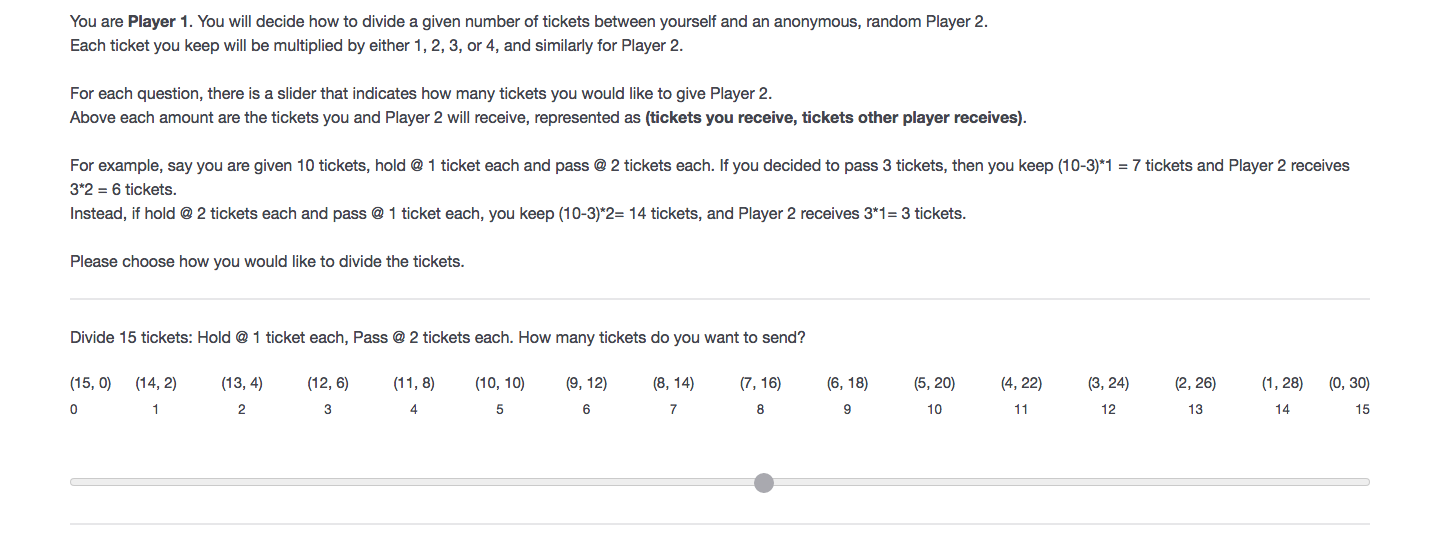
\includegraphics[scale=0.35]{gendict1}\\
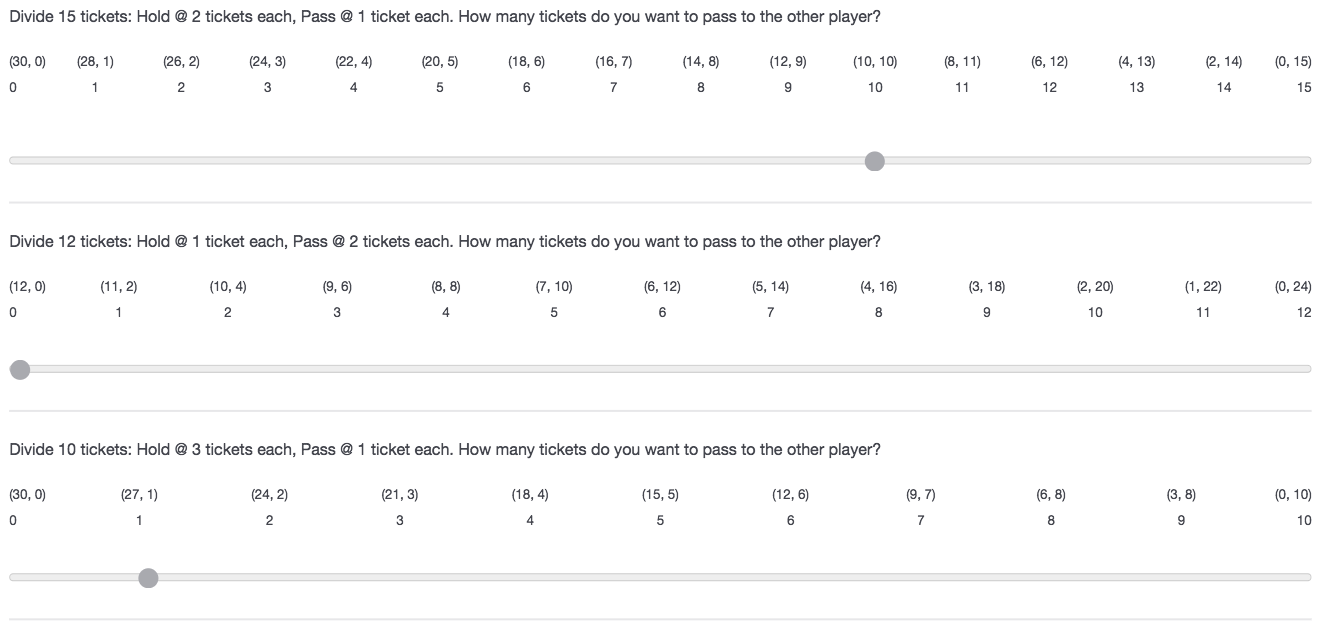
\includegraphics[scale=0.35]{gendict2}\\
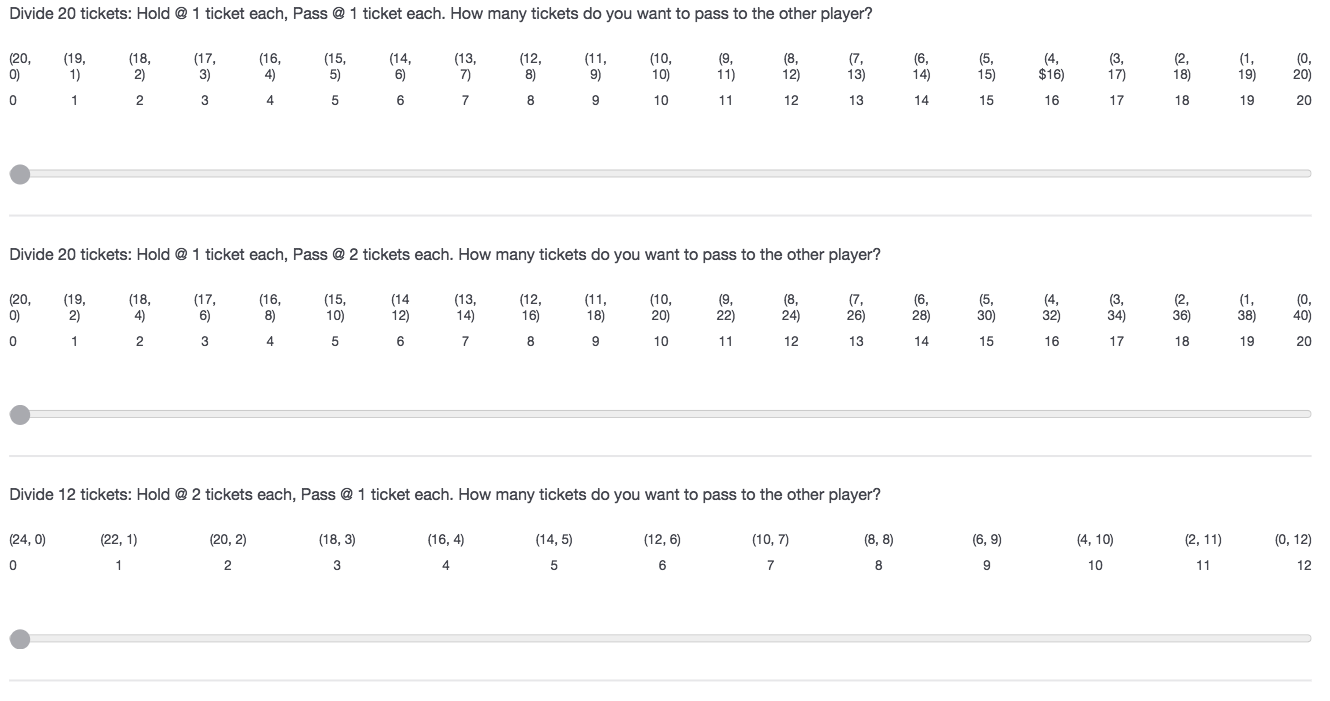
\includegraphics[scale=0.35]{gendict3}\\
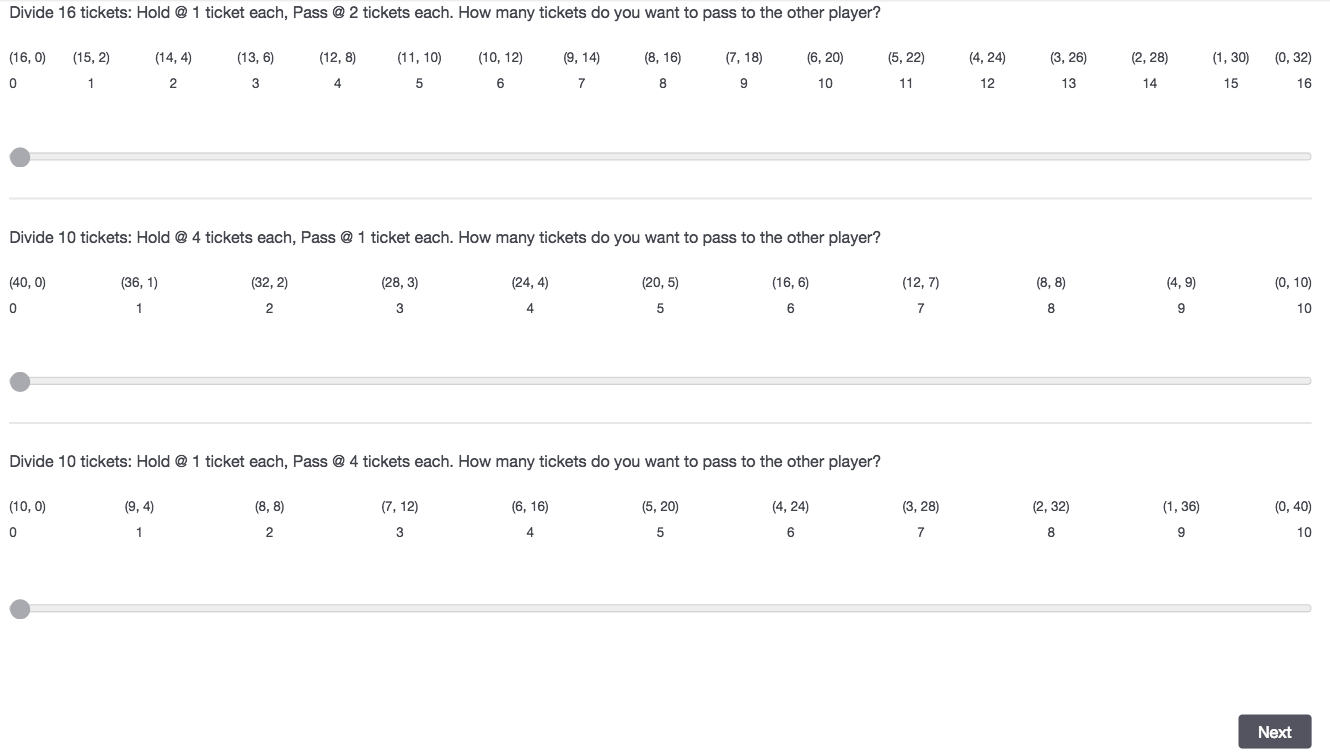
\includegraphics[scale=0.35]{gendict4}\\ \\
\newpage
\begin{center}
Figure C.2: Ultimatum Game Player 1
\end{center}
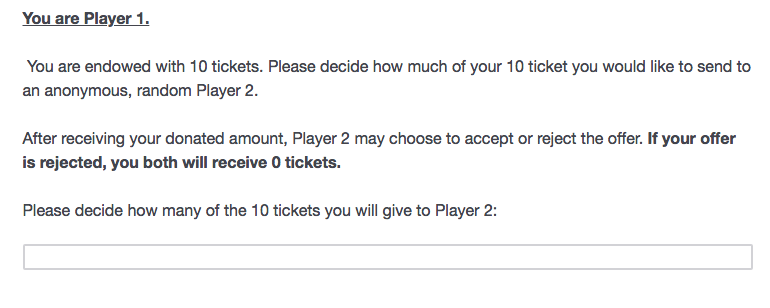
\includegraphics[scale=0.5]{ultimatum1} \\ 
\begin{center}
Figure C.3: Ultimatum Game Player 2 
\end{center}
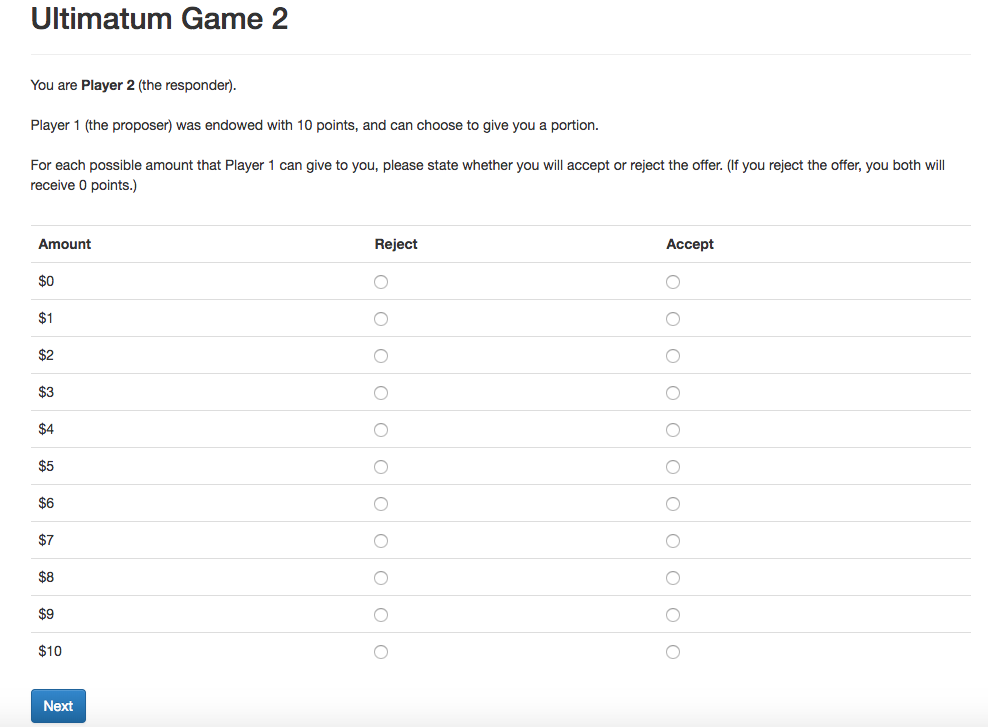
\includegraphics[scale=0.5]{ultimatum2} \\
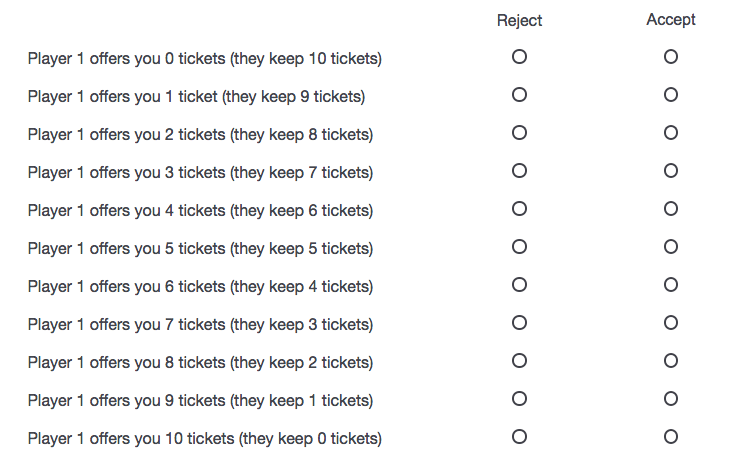
\includegraphics[scale=0.5]{ultimatum3} \\ 
\newpage
\begin{center}
Figure C.4: Trust Game Player 1
\end{center}
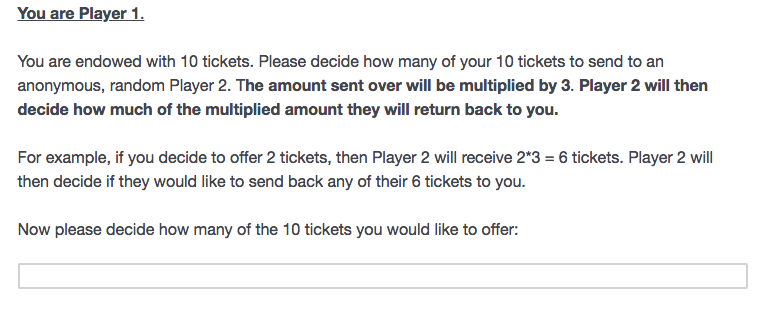
\includegraphics[scale=0.5]{trust1} \\ 
\begin{center}
Figure C.5: Trust Game Player 2
\end{center}
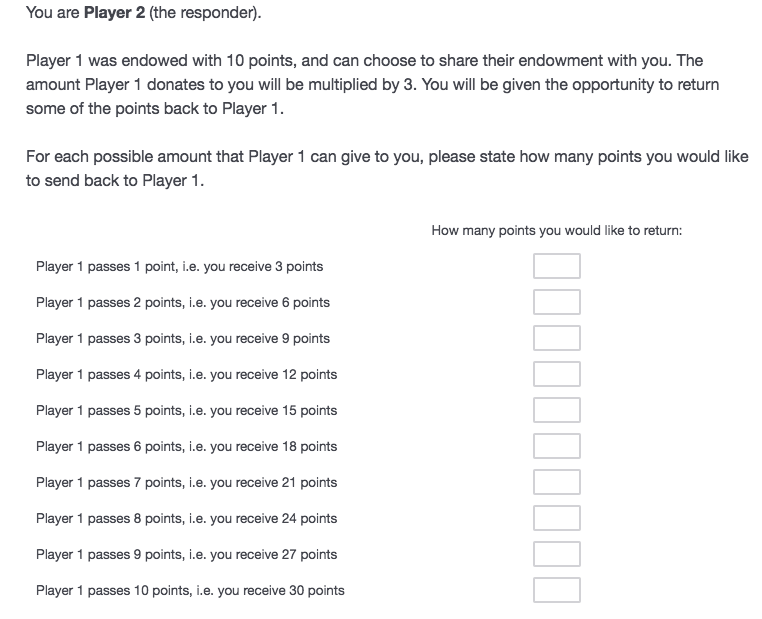
\includegraphics[scale=0.5]{trust2} \\
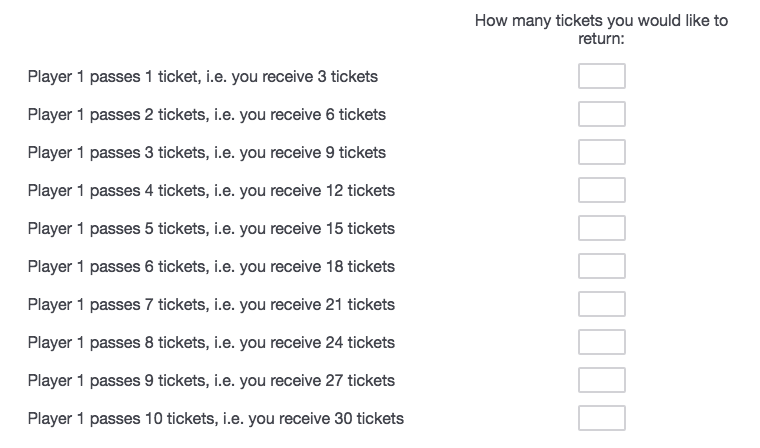
\includegraphics[scale=0.5]{trust3} \\ 
\newpage
\begin{center}
Figure C.6: Public Goods Game
\end{center}
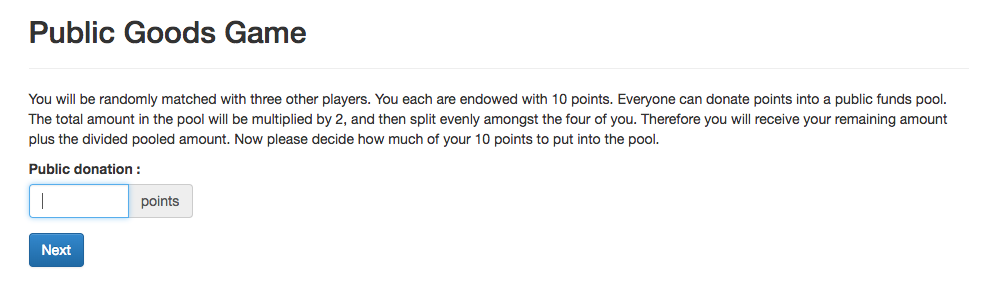
\includegraphics[scale=0.5]{public} \\
\newpage
\section{Self-Report Altruism (SRA) Items}
\vspace{8mm} 

\begin{tabular}{ | p{12cm} | }
\hline

1. I have allowed someone to go ahead of me in line.\\
\hline
2. I have donated money at the cash register when buying groceries.*\\
\hline
3. I have given money to a stranger (or an acquaintance I don\rq t know too well) in need.*\\ 
\hline
4. I have donated to a charity.*\\
\hline
5. I have done volunteer work for a charity/organization.\\
\hline
6. I have delayed an elevator/held door open for stranger(s).\\
\hline
7.  I have pointed out a clerk\rq s error (at a supermarket, restaurant) in undercharging me.*\\
\hline
8. I have gone out of my way to meet with someone to help them with a task (e.g. help proofread their paper, listen to their presentation, etc). \\
\hline
9. I have offered my seat on a bus/train to a stranger who was standing.\\
\hline
10. I have helped an acquaintance with moving in/ moving out of their dorm/apartment/house.\\
\hline
\end{tabular} \\
\small Note: * indicates SRA item is related to money. \\ \\






\end{document}